\documentclass[12pt]{article}
\usepackage{amssymb,amsmath,graphicx,mathtools, tikz, parskip, framed, float, hyperref}
\usepackage{listings}
\usepackage[margin=0.75in]{geometry}
\usepackage{color}
\parindent 16 pt
\usepackage{fancyhdr}
\pagestyle{fancy}

\fancyhead[R]{\footnotesize{Imad Ali\\
Ross Flek}}
\fancyhead[L]{\footnotesize{Vector Calculus Notes \\
Version 1.0
}}
\DeclarePairedDelimiter\ceil{\lceil}{\rceil}
\DeclarePairedDelimiter\floor{\lfloor}{\rfloor}

\lstset{
    language=R,
    basicstyle=\scriptsize\ttfamily,
    stepnumber=1,
    numbersep=5pt,
    showspaces=false,
    showstringspaces=false,
    showtabs=false,
    frame=single,
    tabsize=2,
    captionpos=b,
    breaklines=true,
    breakatwhitespace=false,
    escapeinside={},
    keywordstyle={},
    morekeywords={}
    }
% Remove indentation
\setlength{\parindent}{0pt}

% Title page
\title{\textbf{Vector Calculus Notes}}
\author{Imad Ali \\
Ross Flek}
\date{\today \\
\bigskip
Version 1.0
}

\begin{document}

% CUSTOM SHORTCUTS

\def\ci{\perp\!\!\!\perp}
\def\ex{\mathbb{E}}
\def\prob{\mathbb{P}}
\def\ind{\mathbb{I}}
\def\grad{\triangledown}
\def\bigo{\mathcal{O}}

\def\real{\mathbb{R}}
\def\p#1#2{\frac{\partial #1}{\partial #2}}
\def\norm#1{\parallel#1\parallel}

\maketitle

\tableofcontents

\pagebreak

\section*{Preface}

This document is intended to provide a brief overview of the salient topics in Vector Calculus at the level of a Calculus III/IV course. It is intended to read like a rough set of notes. \\

Most of this document is based off of discussions with Ross Flek with reference to Thomas Barr's \emph{Vector Calculus}. For a more comprehensive discussion of the field see \emph{Vector Calculus} by Thomas Barr (2001) or \emph{Calculus} by James Stewart (2007). For more detail on Linear Algebra see \emph{Introduction to Linear Algebra} by Gilbert Strang (2003). John Baez (\url{http://math.ucr.edu/home/baez/books.html}) also references some books when self-studying Calculus (or most topics in Math and Physics). Particularly, those who have a weak (or no) background in Calculus are advised to start with \emph{Calculus Made Easy} by Silvanus Thompson. It does a great job at providing intuition about the topic at an introductory level. \\ 

This document was complied by Imad Ali (\url{http://imadali.net}) and Ross Flek. Please share any comments, suggestions, and corrections at \url{https://github.com/imadmali/avc}. This document is licensed under \href{https://creativecommons.org/licenses/by-nc-sa/4.0/}{\tt CC BY-NC-SA 4.0}.
 
\pagebreak
 
\section{Linear Algebra}

\subsection{Vectors}

An \emph{n-dimensional} vector is an \emph{n-tuple} of numbers. The values of the tuple are the \emph{components} or \emph{elements} of the vector. A vector is denoted as $\vec{v}$ or $\mathbf{v}$. A \emph{zero vector} or a \emph{null vector} is where all components of the vector are zero. A \emph{unit vector} is a vector that has a \emph{magnitude} or \emph{length} of one (vector length is discussed below). Note that dividing a vector by its magnitude (i.e. $\frac{\vec{v}}{|\vec{v}|})$ will result in a unit vector. \\

In addition to magnitude, vectors can be represented as arrows and give a sense of \emph{direction}. For instance, in two-dimensional space the vector $\vec{p}=(3,5)$ is illustrated by drawing a line from the origin to the point represented by the coordinates $(3,5)$. This is illustrated in Figure ~\ref{fig:vector}.\\

% Vector Multiplication
\begin{figure}[h!]
\centering
\caption{Two Dimensional Vector}
\label{fig:vector}
\begin{tikzpicture}[scale=0.7, every node/.style={scale=0.5}]
% Draw axes
\draw[->,dashed, gray] (-2,0)--(7,0) node[right]{$x$};
\draw[->,dashed, gray] (0,-2)--(0,7) node[above]{$y$};
% Draw tick marks
\foreach \x in {-1,-2,1,2,3,4,5,6,7}
    \draw (\x cm,1pt) -- (\x cm,-1pt) node[anchor=north, gray] {$\x$};
\foreach \y in {-1,-2,1,2,3,4,5,6,7}
    \draw (1pt,\y cm) -- (-1pt,\y cm) node[anchor=east, gray] {$\y$};
% Draw vectors
\draw[->, semithick, black](0,0) -- (3,5);
\end{tikzpicture}
\end{figure}

 There are two operations that can be performed on vectors. 
\begin{itemize}
\item \emph{Scalar multiplication}: An n-dimensional vector $\vec{p}$ can be multiplied by some scalar $a$. The resulting vector $a\vec{p}$ is where every component in $\vec{p}$ is multiplied by $a$.
\[
a\vec{p} = (ap_1, ap_2, \ldots, ap_{n-1}, ap_n)
\]
Scalar multiplication stretches or contracts vector, and can change the direction of a vector.
\item \emph{Summation}: Provided that all vectors have the same dimension, they can be added to create a new vector. Similar to multiplication, addition is done by summing the $n^{th}$ component in one vector with the $n^{th}$ component in another vector. 
\[
\vec{p}+\vec{q} = (p_1 + q_1, p_2 + q_2, \ldots, p_{n-1} + q_{n-1}, p_n + q_n)
\]
\end{itemize}

Vector scalar multiplication is illustrated in Figure~\ref{fig:vectormultiplication} and vector summation is illustrated in Figure~\ref{fig:vectorsummation}. You can see how multiplying a vector by a negative scalar will cause the vector to point in the opposite direction. Multiplying a vector by a scalar less than one will reduce the magnitude of the vector and multiplying by a scalar greater than one will increase the magnitude. With regard to vector summation, notice that the summation of the two vectors creates a vector that is a weighted average of the summed vectors. Graphically, this vector is the diagonal of the parallelogram whose edges are defined by the original vectors. The physical interpretation of the summation of two vectors is that it is the \emph{resultant force} of the two forces prescribed by the two vectors. \\

% Vector Multiplication
\begin{figure}[h!]
\centering
\caption{Vector Multiplication}
\label{fig:vectormultiplication}
\begin{tikzpicture}[scale=0.7, every node/.style={scale=0.5}]
% Draw axes
\draw[->,dashed, gray] (-2,0)--(7,0) node[right]{$x$};
\draw[->,dashed, gray] (0,-2)--(0,7) node[above]{$y$};
% Draw tick marks
\foreach \x in {-1,-2,1,2,3,4,5,6,7}
    \draw (\x cm,1pt) -- (\x cm,-1pt) node[anchor=north, gray] {$\x$};
\foreach \y in {-1,-2,1,2,3,4,5,6,7}
    \draw (1pt,\y cm) -- (-1pt,\y cm) node[anchor=east, gray] {$\y$};
% Draw vectors
\draw[->, semithick, orange](2,2) -- (5,5);
\draw[->, semithick, black](2,2) -- (4,4);
\draw[->, semithick, cyan](2,2) -- (3,3);
\draw[->, semithick, magenta](2,2) -- (-1,-1);
\end{tikzpicture}
\end{figure}

% Vector Summation
\begin{figure}[h!]
\centering
\caption{Vector Summation}
\label{fig:vectorsummation}
\begin{tikzpicture}[scale=0.7, every node/.style={scale=0.5}]
% Draw axes
\draw[->,dashed, gray] (-2,0)--(7,0) node[right]{$x$};
\draw[->,dashed, gray] (0,-2)--(0,7) node[above]{$y$};
% Draw tick marks
\foreach \x in {-1,-2,1,2,3,4,5,6,7}
    \draw (\x cm,1pt) -- (\x cm,-1pt) node[anchor=north, gray] {$\x$};
\foreach \y in {-1,-2,1,2,3,4,5,6,7}
    \draw (1pt,\y cm) -- (-1pt,\y cm) node[anchor=east, gray] {$\y$};
% Draw vectors
\draw[->, semithick, black](-1,1) -- (2,4);
\draw[->, semithick, black](-1,1) -- (3,-2);
\draw[->, dashed, black](2,4) -- (6,1);
\draw[->, semithick, cyan](-1,1) -- (6,1);
% Draw labels
\node [label=left:{(-1,1)}] at (-1,1) {};
\node [label=above:{(2,4)}] at (2,4) {};
\node [label=below:{(3,-2)}] at (3,-2) {};
\node [label=right:{(6,1)}] at (6,1) {};
\end{tikzpicture}
\end{figure}

Note that two nonzero vectors $\vec{p}$ and $\vec{q}$ are \emph{parallel} if one is a scalar multiple of the other. Parallel vectors are often denoted $\vec{p}\parallel\vec{q}$.

The \emph{dot product} (\emph{scalar product} or \emph{inner product}) for two n-dimensional vectors is obtained by multiplying the corresponding components in each vector and then summing across these products. 
\[
\vec{p}\cdot \vec{q} = \vec{q}\cdot \vec{p} = p_1 \cdot q_1 + p_2 \cdot q_2 + \ldots + p_{n-1} \cdot q_{n-1} + p_n \cdot q_n
\]

The dot product measures the extent to which two vectors point in the same direction. The dot product will be positive if they point in the same direction, negative if they point in opposite directions, and zero if they are \emph{orthogonal} (i.e. perpendicular) to each another. Orthogonal vectors are often denoted $\vec{p}\perp\vec{q}$. Note that the dot product of a nonzero vector with itself cannot be zero. The geometric interpretation of this is nonsensical since it would require a vector to be perpendicular to itself. \\

Consider the vector $\vec{p}$. The \emph{magnitude} (also known as the \emph{length} or \emph{norm}) of this vector, denoted $\norm{\vec{p}}$, from its origin is calculated using the \emph{Pythagorean Theorem},
\begin{align*}
\norm{\vec{p}} = \sqrt{p_x^2+p_y^2} = \sqrt{\vec{p}\cdot\vec{p}}
\end{align*}

In this context the origin refers to where the vector starts, which is not necessarily the origin (0,0) in the x-y plane. Notice that the magnitude of a vector is the square root of the dot product of the vector with itself. At the beginning of the section we mentioned the concept of a unit vector. A \emph{unit vector} is a vector that has a norm of one. For example, $\vec{v}=(0,1)$ is a unit vector. As mentioned, and vector divided by its norm results in a unit vector. \\

Figure~\ref{fig:vectorlength} below illustrates the intuition behind finding the length of a vector in $\mathbb{R}^2$ space. \\

\begin{figure}[h!]
\centering
\caption{Vector Length}
\label{fig:vectorlength}
\begin{tikzpicture}[scale=0.7, every node/.style={scale=0.5}]
% Draw axes
\draw[->,dashed, gray] (0,0)--(7,0) node[right]{$x$};
\draw[->,dashed, gray] (0,0)--(0,7) node[above]{$y$};
% Draw tick marks
\foreach \x in {0,1,2,3,4,5,6,7}
    \draw (\x cm,1pt) -- (\x cm,-1pt) node[anchor=north, gray] {$\x$};
\foreach \y in {1,2,3,4,5,6,7}
    \draw (1pt,\y cm) -- (-1pt,\y cm) node[anchor=east, gray] {$\y$};
% Draw vectors
\draw[->, semithick, black](2,2) -- (4,4);
\draw[-, semithick, dotted, black](2,2) -- (4,2);
\draw[-, semithick, dotted, black](4,2) -- (4,4);
\end{tikzpicture}
\end{figure}

Before we show how the dot product of two vectors relates to the angle of those two vectors, we need a way to find the vector that connects two vectors. By definition, let $\vec{v}$ be perpendicular to $\vec{w}$. The vector that connects $\vec{v}$ and $\vec{w}$ is parallel to the vector $\vec{v}-\vec{w}$. See Figure~\ref{fig:vectordistance} for an illustration. If $\vec{v}\perp\vec{w}$ then using the Pythagorean Theorem we have,
\[
\norm{\vec{v}}^2 + \norm{\vec{w}}^2 = \norm{\vec{v}-\vec{w}}^2
\]
Expanding we have,
\begin{align*}
v_1^2 + v_2^2 + w_1^2 + w_2^2 &= v_1^2 - 2v_1w_1 + w_1^2 + v_2^2 - 2v_2w_2 + w_2^2 \\
v_1w_1 + v_2w_2 &= 0
\end{align*}
Therefore, perpendicular vectors produce a dot product $\vec{v}\cdot\vec{w}=0$. \\

Another approach is to define the vectors in terms of angles. In this case let $\vec{u}=(\cos{\theta},\sin{\theta})$ and let $\vec{w}=(\sin{\theta},\cos{\theta})$. When $\theta=90^\circ=\frac{\pi}{2}$ the vectors $\vec{u}$ and $\vec{w}$ are the basis vectors in $\real^2$ and have a $\theta$ angle between them. The dot product $\vec{u}\cdot\vec{w} = 0$, which implies that perpendicular vectors have a dot product equal to zero. \\

\begin{figure}[h!]
\centering
\caption{Vector Distance}
\label{fig:vectordistance}
\begin{tikzpicture}[scale=0.7, every node/.style={scale=0.5}]
% Draw axes
\draw[->,dashed, gray] (0,0)--(7,0) node[right]{$x$};
\draw[->,dashed, gray] (0,0)--(0,7) node[above]{$y$};
% Draw tick marks
\foreach \x in {0,1,2,3,4,5,6,7}
    \draw (\x cm,1pt) -- (\x cm,-1pt) node[anchor=north, gray] {$\x$};
\foreach \y in {1,2,3,4,5,6,7}
    \draw (1pt,\y cm) -- (-1pt,\y cm) node[anchor=east, gray] {$\y$};
% Draw vectors
\draw[->, semithick, black](2,2) -- (4,4);
\draw[->, semithick, black](2,2) -- (6,2);
\draw[-, semithick, cyan](6,2) -- (4,4);
\draw[-, semithick, dashed, cyan](2,2) -- (4,0);
\draw[-, semithick, dotted, black](4,4) -- (6,4);
\draw[-, semithick, dotted, black](6,2) -- (6,4);
\end{tikzpicture}
\end{figure}

 Two vectors whose dot product is zero are said to be \emph{orthogonal} vectors. Graphically, orthogonal vectors are vectors that are perpendicular to one another as seen in Figure~\ref{fig:orgthogonalvectors}. \\

\begin{figure}[h!]
\centering
\caption{Orthogonal Vectors}
\label{fig:orgthogonalvectors}
\begin{tikzpicture}[scale=0.7, every node/.style={scale=0.5}]
% Draw axes
\draw[->,dashed, gray] (0,0)--(7,0) node[right]{$x$};
\draw[->,dashed, gray] (0,0)--(0,7) node[above]{$y$};
% Draw tick marks
\foreach \x in {0,1,2,3,4,5,6,7}
    \draw (\x cm,1pt) -- (\x cm,-1pt) node[anchor=north, gray] {$\x$};
\foreach \y in {1,2,3,4,5,6,7}
    \draw (1pt,\y cm) -- (-1pt,\y cm) node[anchor=east, gray] {$\y$};
% Draw vectors
\draw[->, semithick, black](1,2) -- (4,2);
\draw[->, semithick, black](1,2) -- (1,6);
% Draw perpendicular box
\draw[-, black](1.3,2.3) -- (1.3,2);
\draw[-, black](1.3,2.3) -- (1,2.3);
\end{tikzpicture}
\end{figure}

We have discussed how to interpret the angle of two vectors using the dot product. But what if we want to find the exact angle $\theta$? Consider the basis vector $\vec{i} = (1,0)$ and the vector $\vec{u}=(\cos{\theta}, \sin{\theta})$. The dot product of the two is,
\[
\vec{i}\cdot\vec{u} = \cos{\theta}
\]
This is interesting since it says that $\cos^{-1}(\vec{i}\cdot\vec{u})=\theta$. Unfortunately we are restricting ourself to only basis vectors. To extend this further, let $\vec{v}=(\cos{\alpha},\sin{\alpha})$ and $\vec{u}=(\cos{\beta},\sin{\beta})$, where $\alpha$ and $\beta$ are the angels of $\vec{v}$ and $\vec{u}$, respectively, from the same basis vector such that $\beta-\alpha=\theta$ the angle between $\vec{v}$ and $\vec{u}$. The dot product of the two vectors results in,
\[
\vec{u}\cdot\vec{v} = \cos{\beta}\cos{\alpha} + \sin{\beta}\sin{\alpha}
\] 
Using trigonometric identities we have,
\begin{align*}
\vec{u}\cdot\vec{v} &= \frac{1}{2}\left[ \cos{(\beta-\alpha)} + \cos{(\beta+\alpha)} \right]
+ \frac{1}{2}\left[ \cos{(\beta-\alpha)} - \cos{(\beta+\alpha)} \right] \\
&= \cos{\beta-\alpha} \\
&= \cos{\theta}
\end{align*}

Since the cosine function is bound between -1 and 1, we have.
\[
-1 \leq \cos{\theta} \leq 1
\]

This result tells us that the dot product of any two nonzero unit vectors is bound between -1 and 1. Furthermore, applying $\cos^{-1}(\cdot)$ gives us the angle $\theta$ between the two vectors. \\

Generalizing this further, if $\vec{v}$ and $\vec{u}$ were not unit vectors, we could transform them into unit vectors by dividing them by their respective norms. This would give us the \emph{cosine formula},
\[
\frac{\vec{u}\cdot\vec{v}}{\norm{\vec{u}}\norm{\vec{v}}} = \cos{\theta}
\]
Written in terms of inequalities we have,
\begin{align*}
-1 \leq &\frac{\vec{u}\cdot\vec{v}}{\norm{\vec{u}}\norm{\vec{v}}} \leq 1 \\
-\norm{\vec{u}}\norm{\vec{v}} \leq &\vec{u}\cdot\vec{v} \leq \norm{\vec{u}}\norm{\vec{v}}
\end{align*}
Applying the absolute value and since, by definition, the norm must be positive we have,
\[
|\vec{u}\cdot\vec{v}| \leq \norm{\vec{u}}\norm{\vec{v}}
\]
This is known as the $\emph{Cauchy-Schwartz Inequality}$. The Cauchy-Schwartz Inequality and the cosine formula are identical statements and state that the dot product of two vectors (in unit vector form) cannot exceed 1. \\

We can think of the angle between two vectors as representing how similar the vectors are to one another. An application of the dot product representing the similarity between two vectors can been seen in recommendation systems. Consider $i=1,\ldots,k$ consumers of various products. Each consumer has an n-dimensional vector $\vec{v_i}$ that represents the quantity of each of the $n$ products that have been consumed. In order to make recommendations to a consumer we determine which consumers have similar vectors based on the methods described above. We then make recommendations to that consumer based on what the other consumers have purchased. \\

A function $f(\cdot)$ is a \emph{linear transformation} if it satisfies the following properties.
\begin{itemize}
\item Scalar multiplication: for any vector $\vec{v}$ and any scalar $a$, $f(a\cdot\vec{v})=a\cdot f(\vec{v})$ 
\item Vector addition: for any vectors $\vec{v}$ and $\vec{w}$, $f(\vec{v}+\vec{w}) = f(\vec{v})+f(\vec{w})$ \\
\end{itemize}

More briefly this is saying that $f(a\vec{v}+a\vec{w}=af(\vec{v})+af(\vec{w})$. \\

If a function $f(\cdot)$ is a linear transformation from n-dimensional vectors to numbers, then there exists a unique vector $\vec{u}$ such that, for all $\vec{v}$, $f(\vec{v}) = \vec{u}\cdot\vec{v}$. This is essentially saying that there is some vector $\vec{u}$ that represents the linear transformation that $f(\cdot)$ applies to $\vec{v}$. \\

The concept also applies to matrices. Just like functions apply transformations to their inputs, the product $\mathbf{M}\vec{v}$ transforms $\vec{v}$ into another vector. $\vec{v}$ was the input and the output is $\mathbf{M}\vec{v}$. \\

If one vector can be written as a scalar multiple of another, then both vectors are said to be \emph{linearly dependent}. If both vectors are not linearly dependent, then they are \emph{linearly independent}. This also applies to matrices. It is important since it pertains to dimensionality. Briefly, the dimensions of a set of vectors in $\real^n$ (i.e. a matrix with $n$ rows) is equal to the number of linearly independent vectors. \\
 
For example, consider three vectors in $\real^n$. If one of the vectors can be written as a linear combination as one other vector, then there exists one vector that is linearly independent and two vectors that are linearly dependent. This means that these three vectors exist in $\real^2$ (i.e. two dimensional space) since one vector is a linear combination of the other. \\ 

Vectors have a \emph{magnitude} and a \emph{direction}. When drawing a vector the arrow indicates the direction. The magnitude is calculated using the Pythagorean theorem. Two vectors are identical if they have the same magnitude and direction. A zero vector has no direction and has a magnitude of zero. Both $(0,0)$ and $(0,0,0)$ are zero vectors in the two- and three-dimensional space, respectively A unit vector will have some direction and will have a magnitude of one. Both $(0,1)$ and $(0,1,0)$ are unit vectors in the two- and three- dimensional space, respectively. \\

Consider two vectors $\vec{v}$ and $\vec{w}$. The \emph{vector projection} of $\vec{w}$ onto $\vec{v}$ is obtained by dropping a perpendicular from the head of $\vec{w}$ to the line on which $\vec{v}$ lies, and drawing a vector from the tail of $\vec{v}$ to the point at which the perpendicular intersects the line on which $\vec{v}$ lies. Note that ``perpendicular'' refers to the line being perpendicular with $\vec{v}$ not with $\vec{w}$.\\

The projection, $\vec{p}$, of $\vec{w}$ onto $\vec{v}$ is defined as,
\[
\vec{p} = \frac{\vec{v}\cdot\vec{w}}{\vec{v}\cdot\vec{v}}\vec{v}
\]

Figure~\ref{fig:projection} provides an graphical illustration of two projections. The projection of$\vec{w}=(2,3)$ onto $\vec{v}=(6,2)$ is $\vec{p_1}$, and the projection of $\vec{w}$ onto the x-axis is $\vec{p_2}$.

\begin{figure}[h!]
\centering
\caption{Vector Projection}
\label{fig:projection}
\begin{tikzpicture}[scale=1, every node/.style={scale=0.5}]
% Draw axes
\draw[->,dashed, gray] (0,0)--(7,0) node[right]{$x$};
\draw[->,dashed, gray] (0,0)--(0,4) node[above]{$y$};
% Draw tick marks
\foreach \x in {0,1,2,3,4,5,6,7}
    \draw (\x cm,1pt) -- (\x cm,-1pt) node[anchor=north, gray] {$\x$};
\foreach \y in {1,2,3,4}
    \draw (1pt,\y cm) -- (-1pt,\y cm) node[anchor=east, gray] {$\y$};
% Draw vectors
\draw[->, semithick, black](0,0) -- (2,3) node[right]{$\vec{w}$};
\draw[->, semithick, black](0,0) -- (6,2) node[right]{$\vec{v}$};
\draw[->, thick, cyan](0,0) -- (27/10,9/10) node[below right]{$\vec{p_1}$};
\draw[->, thick, magenta](0,0) -- (2,0) node[above right]{$\vec{p_2}$};
% Draw perpendicuars
\draw[-, dashed, black](2,3) -- (27/10,9/10);
\draw[-, dashed, black](2,3) -- (2,0);
\end{tikzpicture}
\end{figure}

Some authors define projection in terms of the component of a vector. The \emph{component} of $\vec{w}$ in the direction of $\vec{v}$ is the scalar that can transform $\vec{v}$ into the projection of $\vec{w}$ on $\vec{v}$. 
\begin{align*}
comp_{\vec{v}}(\vec{w}) &= \frac{\vec{v}\cdot\vec{w}}{\norm{\vec{v}}} \\
\vec{proj}_{\vec{v}}(\vec{w}) &= comp_{\vec{v}}(\vec{w})\frac{\vec{v}}{\norm{\vec{v}}}
\end{align*}

Note that the projection is a vector and the component is the magnitude of the vector. Substituting the component of $\vec{w}$ into the projection of $\vec{w}$ onto $\vec{v}$ and noting that $\norm{\vec{v}}\norm{\vec{v}}=\vec{v}\cdot\vec{v}$ yields the definition provided above. \\

We previously defined the product of a matrix and a vector as being a linear transformation of the vector. In the context of projection, we can define a \emph{projection matrix} that projects $\vec{w}$ onto another vector. A projection matrix is defined as,
\[
\mathbf{P} = \frac{\vec{v}\cdot\vec{v}^\top}{\vec{v}\cdot\vec{v}}
\]
where $\vec{v}$ is the vector that $\vec{w}$ is being projected onto. To find the projection vector we multiply the projection matrix by the vector being projected: $\mathbf{P}\vec{w}$. Note that $\vec{v}$ is an $n\times1$ vector, which makes $\vec{v}^T$ a $1\times n$ vector. \\

Using the projection of $\vec{w}$ onto the x-axis in the example above, our $\vec{v}=(1,0)$ which gives the following projection matrix,
\[
\mathbf{P} =
\begin{bmatrix}
1 & 0 \\
0 & 0
\end{bmatrix}
\]

So to project $\vec{w}$ onto the x-axis we just need to evaluate $\mathbf{P}\vec{w}=(2,0)$, which gives us the same answer as above. In fact, this projection matrix has the ability to project any two-dimensional vector onto the x-axis.\\

The \emph{cross product} of two nonzero, nonparallel vectors is the vector that is orthogonal to both of them. Given the nonzero, nonparallel vectors $\vec{a}$ and $\vec{b}$, vector $\vec{x}=(x,y,z)$ must be nonzero and satisfy
\begin{align*}
\vec{x}\cdot\vec{a} &= a_1x+a_2y+a_3z = 0 \\
\vec{x}\cdot\vec{b} &= b_1x+b_2y+b_3z = 0
\end{align*}

 Solving this system yields
\[
\vec{x} = (a_2b_3-a_3b_2, a_3b_1-a_1b_3, a_1b_2-a_2b_1)
\]

 We can also find the cross product of two vectors using cofactor expansion. This uses the basis vectors. For instance, the cross product of the three dimensional vectors $\vec{a}$ and $\vec{b}$ can be written as the following,
\[
\vec{a}\times\vec{b} = 
\begin{vmatrix}
\mathbf{i} & \mathbf{j} & \mathbf{k} \\
 a_1 & a_2 & a_3 \\
 b_1 & b_2 & b_3 \\
\end{vmatrix}
=
\begin{vmatrix}
a_2 & a_3 \\
b_2 & b_3
\end{vmatrix}
\mathbf{i}
-
\begin{vmatrix}
a_1 & a_3 \\
b_1 & b_3
\end{vmatrix}
\mathbf{j}
+
\begin{vmatrix}
a_1 & a_2 \\
b_1 & b_2
\end{vmatrix}
\mathbf{k}
\]
where each determinant is a component in the resulting cross product vector. The determinant and basis vectors are covered in more detail below.\\

\subsection{Matrices}

An $m\times n$ \emph{matrix} is an array of elements (e.g. numbers) that contains $m$ rows and $n$ columns. It can also be defined as collection of $m$ n-dimensional vectors or $n$ m-dimensional vectors. Matrices are typically denoted as capital letters, such as $M$ or $\mathbf{M}$. Here we will stick to the boldface type convention. The element corresponding to the $i$th row and the $j$th column of a matrix $\mathbf{M}$ is denoted $\mathbf{M}_{ij}$ or $\mathbf{M}[i,j]$. (The latter notation is typical of most computer programing languages.) An $m\times m$ matrix is known as a \emph{square matrix}. \\

A $3\times3$ matrix is given below.
\[
\mathbf{M}_{3\times3}=
\begin{bmatrix}
  m_{1,1} & m_{1,2} & m_{1,3} \\
  m_{2,1} & m_{2,2} & m_{2,3} \\
  m_{3,1} & m_{3,2} & m_{3,3} 
 \end{bmatrix}
 \]

The transpose of a matrix, denoted $\mathbf{M}^\top$, consists of transforming the rows of $\mathbf{M}$ into the columns of  $\mathbf{M}^\top$ in sequence (starting with the first row becoming the first column). If $\mathbf{M}$ is an $m\times n$ matrix then $\mathbf{M}^\top$ will be a $n\times m$ matrix. A \emph{symmetric matrix} is a square matrix that equals its transpose: $\mathbf{M}=\mathbf{M}^\top$. Below is an example of a non-square matrix and its transpose.\\
\[
\mathbf{M}_{2\times 3}=
\begin{bmatrix}
  m_{1,1} & m_{1,2} & m_{1,3} \\
  m_{2,1} & m_{2,2} & m_{2,3} 
 \end{bmatrix}
 \]
 \[
 \mathbf{M}^\top_{3\times 2}=
\begin{bmatrix}
  m_{1,1} & m_{2,1}  \\
  m_{1,2} & m_{2,2}  \\
  m_{1,3} & m_{2,3}   
 \end{bmatrix}
 \]

Scalar multiplication on matrices and the summation of two matrices is performed component by component, as with vectors. \\

Let $\mathbf{M}$ be an $m\times n$ matrix and $\vec{v}$ be an n-dimensional vector. The product $\mathbf{M}\cdot\vec{v}$ is an m-dimensional vector. The product vector will consist of the dot product of each row of $\mathbf{M}$ and $\vec{v}$. This can also be thought of as a weighted sum of the columns of $\mathbf{M}$ where the weights for each column are the components of $\vec{v}$. The following properties hold for multiplying a matrix by a vector where $\mathbf{M}$ and $\mathbf{N}$ are $m\times n$ matrices, $\vec{u}$ and $\vec{v}$ are n-dimensional vectors, and $a$ is a scalar.
\begin{align*}
(\mathbf{M}+\mathbf{N})\vec{v} &= \mathbf{M}\vec{v}+\mathbf{N}\vec{v} \\
\mathbf{M}(\vec{u}+\vec{v}) &= \mathbf{M}\vec{v} + \mathbf{M}\vec{u} \\
a(\mathbf{M})\vec{v} &= a(\mathbf{M}\vec{v}) = \mathbf{M}(a\vec{v})
\end{align*}

In the previous section we briefly talked about how a matrix can represent a linear transformation. Let $f(\cdot)$ be a function that represents a linear transformation from $\mathbb{R}^n$ to $\mathbb{R}^m$. Then there exists a unique $m\times n$ matrix $\mathbf{F}$ such that, for all $\vec{v}$, $f(\vec{v})=\mathbf{F}\vec{v}$. We say that matrix $\mathbf{F}$ corresponds to the transformation of $f(\cdot)$, and vice versa. For example, the projection matrix can be thought of as a transformation of taking one vector and projecting it onto another. \\

Matrices can represent systems of equations. An example is given below where $\vec{x}$ denotes a n-dimensional vector of unknown variables, $\mathbf{B}$ is a matrix of constants, and $\vec{a}$ is a m-dimensional vector of constants. 
\[
\mathbf{B} = 
\begin{bmatrix}
  b_{1,1} & \ldots & b_{1,n} \\
  \vdots &  & \vdots \\
  b_{m,1} & \ldots & b_{m,n}
 \end{bmatrix}
 \vec{x} = 
 \begin{bmatrix}
 x_{1} \\
 \vdots \\
 x_{n}
 \end{bmatrix}
 \vec{a} = 
 \begin{bmatrix}
 a_{1} \\
 \vdots \\
 a_{m}
 \end{bmatrix}
\]
\[
\begin{bmatrix}
  b_{1,1} & \ldots & b_{1,n} \\
  \vdots &  & \vdots \\
  b_{m,1} & \ldots & b_{m,n}
 \end{bmatrix}
\cdot
 \begin{bmatrix}
 x_{1} \\
 \vdots \\
 x_{n}
 \end{bmatrix}
 = 
 \begin{bmatrix}
 a_{1} \\
 \vdots \\
 a_{n}
 \end{bmatrix}
 =
 \begin{bmatrix}
 b_{1,1} x_{1} + b_{1,2} x_{2} + \ldots + b_{1,n-1} x_{n-1} + b_{1,n} x_{n} = a_{1}\\
  b_{2,1} x_{1} + b_{2,2} x_{2} + \ldots + b_{2,n-1} x_{n-1} + b_{2,n} x_{n} = a_{2} \\
  \vdots \\
   b_{m,1} x_{1} + b_{m,2} x_{2} + \ldots + b_{m,n-1} x_{n-1} + b_{m,n} x_{n} = a_{m}
 \end{bmatrix}
 \]

As mentioned, matrices can be thought of as a collection of vectors. Consider an n-dimensional vector $\vec{v}$ as a $n\times1$ matrix $\mathbf{V}$ and a $m\times n$ matrix $\mathbf{M}$. The product $\mathbf{M}\mathbf{V}$ is a m-dimensional vector in which each component is the dot product between each row of $\mathbf{M}$ and $\mathbf{V}$. Now consider a $n\times m$ matrix $\mathbf{U}$. The product $\mathbf{M}\mathbf{U}$ is a $m\times m$ matrix where each component represents the dot product between each row in $\mathbf{M}$ and each column in $\mathbf{M}$. \\

Given the above we can specify the following. Let $\mathbf{M}$ be a $m\times n$ matrix and $\mathbf{O}$ is a $n \times p$ matrix. The product $\mathbf{M}\mathbf{O}$ is a $m\times p$ matrix whose $i,k$ elements are defined by,
\[
\mathbf{M}\mathbf{O}_{i,k} = \mathbf{M}_{i,.} \cdot \mathbf{O}_{.,k}
\] 
where $\mathbf{M}_{i,.} \cdot \mathbf{O}_{.,k}$ is the dot product of the $i$th row in $\mathbf{M}$ and the $j$th column in $\mathbf{O}$. \\

A few special matrices include the \emph{identity matrix} and \emph{triangular matrices}. An identity matrix is a symmetric matrix (i.e. a square matrix that possesses symmetry along the main diagonal) where the components along the main diagonal are all equal to one. It has the ability to preserve the identity of the matrix that is being multiplied by it (similar to the property of the product between the number 1 and scalars). Consider the $m\times n$ matrix $\mathbf{M}$. Then there exists two identity matrices, $\mathbf{I}_{n}$ and $\mathbf{I}_{m}$, that will preserve the $\mathbf{M}$ when multiplied on the right and left sides, respectively. Below is an example using a $3\times2$ matrix. 
\[
\begin{bmatrix}
a & b \\
c & d \\
e & f
\end{bmatrix}
\cdot
\begin{bmatrix}
1 & 0 \\
0 & 1 
\end{bmatrix}
=
\begin{bmatrix}
a & b \\
c & d \\
e & f
\end{bmatrix}
\mbox{and\ } 
\begin{bmatrix}
1 & 0 & 0 \\
0 & 1 & 0 \\
0 & 0 & 1
\end{bmatrix}
\cdot
\begin{bmatrix}
a & b \\
c & d \\
e & f
\end{bmatrix}
=
\begin{bmatrix}
a & b \\
c & d \\
e & f
\end{bmatrix}
\]

A \emph{upper triangular matrix} is a square matrix where all the components below the main diagonal are zero. A \emph{lower triangular matrix} is a square matrix where all the components above the main diagonal are zero. The transpose of an upper triangular matrix is a lower triangular matrix (and vice versa). \\

The \emph{determinant} of a $2\times2$ matrix is the product of the components on the main diagonal minus the product of the components on the off diagonal.
\[
det(\mathbf{A})=
\begin{vmatrix}
a_1 & a_2 \\
b_1 & b_2
\end{vmatrix}
= a_1 b_2 - a_2 b_1
\]

The determinant of a $3\times3$ matrix utilizes that determinant of $2\times2$ matrices and is defined as,
\[
\begin{vmatrix}
a_1 & a_2 & a_3\\
b_1 & b_2 & b_3 \\
c_1 & c_2 & c_3
\end{vmatrix}
=
a_1
\begin{vmatrix}
b_2 & b_3 \\
c_2 & c_3
\end{vmatrix}
- a_2
\begin{vmatrix}
b_1 & b_3 \\
c_1 & c_3
\end{vmatrix}
+ a_3
\begin{vmatrix}
b_1 & b_2 \\
c_1 & c_2
\end{vmatrix}
\]

Higher order matrices can be solved by breaking them up into smaller constituent parts, as done with the $3\times3$ matrix. \\

A $m\times m$ square matrix $\mathbf{A}$ is \emph{invertible} if there exists an $m\times m$ square matrix $\mathbf{B}$ such that $\mathbf{BA}=\mathbf{I}_m$ and $\mathbf{AB}=\mathbf{I}_m$. In this context $\mathbf{B}=\mathbf{A}^{-1}$ is the inverse of $\mathbf{A}$, and vice versa. Note that this definition implies that the inverse of an invertible matrix is unique (i.e. the right inverse and the left inverse are the same matrix). (The concept of the inverse in matrix algebra is similar to the scalar concept: a scalar $\alpha$ times its inverse $\frac{1}{\alpha}$ equals 1.)\\

The inverse for any square $2\times2$ matrix $\mathbf{A}$ is a matrix that contains the negative of the components on the off diagonal and swaps the components on the main diagonal of the original matrix $\mathbf{A}$ divided by the determinant of the original matrix. An example follows,
\[
\mathbf{A}=
\begin{bmatrix}
a & b \\
c & d
\end{bmatrix}
\]
\[
\mathbf{A}^{-1}=
\frac{1}{det(\mathbf{A})}
\begin{bmatrix}
d & -b \\
-c & a
\end{bmatrix}
\]
In order for a matrix to be invertible, we also require that the determinant is not equal to zero. The matrix that is being multiplied by the factor $\frac{1}{det(\mathbf{A})}$ is known as the \emph{adjoint} of $\mathbf{A}$, denoted $adj(\mathbf{A})$. In the context of the example above,
\[
adj(\mathbf{A}) = 
\begin{bmatrix}
d & -b \\
-c & a
\end{bmatrix}
\]

If two matrices $\mathbf{A}$ and $\mathbf{B}$ are invertible, then their product $\mathbf{AB}$, if it exists, is also invertible. Specifically,
\[
(\mathbf{AB})^{-1} = \mathbf{B}^{-1}\mathbf{A}^{-1}
\]

\subsection{Vector Space}
\emph{Vector spaces} are certain sets of n-dimensional vectors. Specifically, they are vectors that can undergo vector addition and scalar multiplication. A \emph{subspace} of $\mathbb{R}^n$ is a particular type of set of n-dimensional vectors. Subspaces of $\mathbb{R}^n$ are a type of vector space. \\

A \emph{linear combination} of a set of vectors $\vec{v}_1,\vec{v}_2,\ldots,\vec{v}_n$ in $\mathbb{R}^n$ is the sum of these vectors scaled by some constants from $\mathbb{R}$: $c_1\vec{v}_1+c_2\vec{v}_2+\ldots+c_n\vec{v}_n$. These are \emph{linear} combinations since we are simply adding the vectors and then scaling them up by some constant (we are not multiplying vectors by one another). \\

There are vectors whose linear combination can represent any vector in the predefined space. These vectors are known as \emph{basis vectors}. In $\real^2$ the basis vectors are $(1,0)$ and $(0,1)$ and are often denoted $\mathbf{i}=(1,0)$ and $\mathbf{j}=(0,1)$. We can write any vector $\vec{v}\in\real^2$ as a linear combination of these basis vectors,
\begin{align*}
\vec{v} &= c_1\mathbf{i} + c_2\mathbf{j} \\
(v_1,v_2) &= c_1(1,0) + c_2(0,1)
\end{align*}

In $\real^3$ the basis vectors are $\mathbf{i} = (1,0,0)$, $\mathbf{j} = (0,1,0)$, and $\mathbf{k} = (0,0,1)$. In $\real^n$ the $n^{th}$ basis vector has a 1 in the $n^{th}$ place and zeros ever where else. \\

The set of all of the vectors that can be represented in $\mathbb{R}^n$ by all the possible linear combinations on $\vec{v}_1,\vec{v}_2,\ldots,\vec{v}_n$ is denoted $span(\vec{v}_1,\vec{v}_2,\ldots,\vec{v}_n)$. Specifically, this represents the set of sum of all the possible scaled combinations of the vectors. Mathematically,
\[
span(\vec{v}_1,\vec{v}_2,\ldots,\vec{v}_n) = \{ c_1\vec{v}_1+c_2\vec{v}_2+\ldots+c_n\vec{v}_n\ |\ c_i \in \mathbb{R}^n\ \forall\ 1 \leq i \leq n \}
\]

To determine the span of a set of vectors you have to solve the system of equations,
\[
c_1\vec{v}_1+c_2\vec{v}_2+\ldots+c_n\vec{v}_n\ = x_n
\]
for the constants.

A few important cases:
\begin{itemize}
\item $span(0)=0$
\item Let $\vec{v}_1$ and $\vec{v}_2$ be orthogonal 2-dimensional vectors. Then $span(\vec{v}_1,\vec{v}_2)=\mathbb{R}^2$.\\
\end{itemize} 

The \emph{plane through point $x = (x_0,y_0,z_0)$ perpendicular to nonzero vector $\vec{n}=(n_1,n_2, n_3)$} consists of all points $x=(x,y,z)$, such that $(x-x_0)\cdot \vec{n} = 0$. The vector $\vec{n}$ is called a \emph{normal} to the plane.  The equation for the plane will take the following form.
\[
n_1(x-x_0)+n_2(y-y_0)+n_3(z-z_0)=0
\]

Given a vector $\vec{m}$ and point $x_0=(x_0,y_0,z_0)$ we define the \emph{line through $x_0$ parallel to $\vec{m}$} to be the set
\[
\{x\in\mathbb{R}^3|x=t\vec{m}+x_0, t\in\mathbb{R}\}
\]

$\vec{m}$ is known as the \emph{direction vector} of the line. The vector equation $x=t\vec{m}+x_0$ is known as the \emph{parametrization} of the line where the \emph{parameter} is $t$. Since $x$ is a set of three-dimensional coordinates we can obtain the following \emph{parametric equations} for the line:
\begin{align*}
x &= n_1t + x_0 \\
y &= n_2t + y_0 \\
z &= n_3t +z_0
\end{align*}

Consider a linear transformation $T:\mathbb{R}^n\rightarrow\mathbb{R}^n$. If we apply $T$ to the collection of points $P$ in $\mathbb{R}^n$ then we will obtain a new collection of points $T(P)=\{ T(x)|x\in P \}$. $T(P)$ is known as the \emph{image of $P$ under $T$}. A linear transformation of $T$ on $\mathbb{R}^n$ is called a \emph{dilation} if $T(x)=rx$ for some $r\in\mathbb{R}^n$. Dilation is a special case of \emph{coordinate rescaling}. Coordinate rescaling involves a linear transformation of the form $T(x)=\mathbf{D}x$ where $\mathbf{D}$ is a diagonal matrix.  \\

Consider $\mathbb{R}^n$ to be the space containing the n-dimensional vectors $\vec{v}_1,\vec{v}_2,\ldots,\vec{v}_n$. More formally, The set of vectors $V=\{\vec{v}_1,\vec{v}_2,\ldots,\vec{v}_n\}\in\mathbb{R}^n$. The set of vectors $V$ is a \emph{subspace} of $\mathbb{R}^n$ if the following three conditions hold:
\begin{enumerate}
\item $V$ contains the zero vector, $\mathbf{0}$. 
\item For any vector $\vec{x}$ in $V$ and any scalar $a$, $a\vec{x}$ must also be in $V$.
\item For any vectors $\vec{x}$ and $\vec{y}$ in $V$, the sum $\vec{x}+\vec{y}$ must also be in $V$. \\
\end{enumerate}

Point 2 refers to the subspace being closed under scalar multiplication and point 3 refers to the subspace being closed under addition.

\subsection{Eigendecomposition}

An \emph{eigendecomposition} is the decomposition of a matrix into its constituent parts: \emph{eigenvalues} and \emph{eigenvectors}.\\

Consider the linear transformation $T:\mathbb{R}^n\rightarrow\mathbb{R}^n$. Given the linear transformation $T$ there exists at most n vectors $\vec{v}\in\mathbb{R}^n$ such that $T(\vec{v})=\lambda_n \vec{v}$, where $\lambda$ is some scalar that transforms $\vec{v}$. Here, $\vec{v}$ is known as the eigenvector for the transformation $T$ and $\lambda$ is the eigenvalue associated with the eigenvector $\vec{v}$.

More formally, if you have a matrix $\mathbf{A}$ that represents some linear transformation then we have,
\[
\lambda\vec{v}=\mathbf{A}\vec{v}
\]
where $\vec{v}$ is the eigenvector of $\mathbf{A}$ and $\lambda$ is the eigenvalue associated with the eigenvector $\vec{v}$. \\

We can solve for the eigenvectors and eigenvalues by using the identity $\vec{v}=\mathbf{I}_n\vec{v}$.
\begin{align*}
\lambda\vec{v}-\mathbf{A}\vec{v} &= \mathbf{0} \\
\lambda\mathbf{I}_n\vec{v}-\mathbf{A}\vec{v}&= \mathbf{0} \\
(\lambda\mathbf{I}_n-\mathbf{A})\vec{v} &= \mathbf{0}
\end{align*}

$\mathbf{A}\vec{v}=\lambda\vec{v}$ for nonzero $\vec{v}$ if and only if the determinant of $\lambda\mathbf{I}_n-\mathbf{A}$ is zero. \\


\pagebreak
\section{Equations of Lines and Planes}

Here we generalize the equation of a line to three-dimensional space and introduce the equation of a plane in three-dimensional space. \\

 An intuitive way to understand the equation of a line in $\mathbb{R}^3$ is by example. Suppose we want to graph the value $x=6$ in $\mathbb{R}$, $\mathbb{R}^2$, or $\mathbb{R}^3$.
\begin{itemize}
\item In $\mathbb{R}$ it will just be a point where $x=6$.
\item In $\mathbb{R}^2$ it will be a vertical line that crosses the x-axis at $x=6$. This line will consider all the potential $y$ coordinates at $x=6$. We can write this as $(6,y)$ for all $y\in\mathbb{R}$. Formally, we can say that the equation of this line is $a6+by=c\implies y=c-6$.
\item In $\mathbb{R}^3$ it will be a plane. This follows naturally from the description in $\mathbb{R}^2$. We are considering all the potential $z$ coordinates \emph{and} all the potential $y$ coordinates such that $x=6$. More formally, we are considering $(6,y,z)$ for all $y,z\in\mathbb{R}$. Note that a plane is a special case of a surface where at least one of the coordinates is fixed (in this case $x$).
\end{itemize}

 What about a familiar equation for a line $y=3x+9$ in $\mathbb{R}^2$ or $\mathbb{R}^3$.
\begin{itemize}
\item In $\mathbb{R}^2$ it will be a line. Passing any $x$ value into the function will give you a corresponding $y$ value and will allow you to trace out the function in two-dimensional space.
\item In $\mathbb{R}^3$ this will be a plane. In $\mathbb{R}^2$ the equation traces out a line when a sequence of $x$ values is passed into it. This exists for all $z\in\mathbb{R}$. So we are using the line to trace out a plane for every value of $z$. 
\end{itemize}

\begin{figure}[H]
\centering
\caption{Two and Three Dimensional Plots of $y=3x+9$}
\label{fig:eq_line}
\indent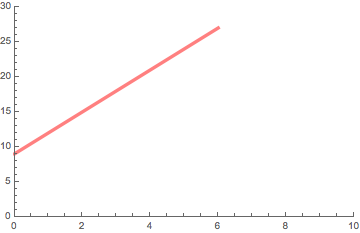
\includegraphics[scale=0.6]{eq_line.png}
\indent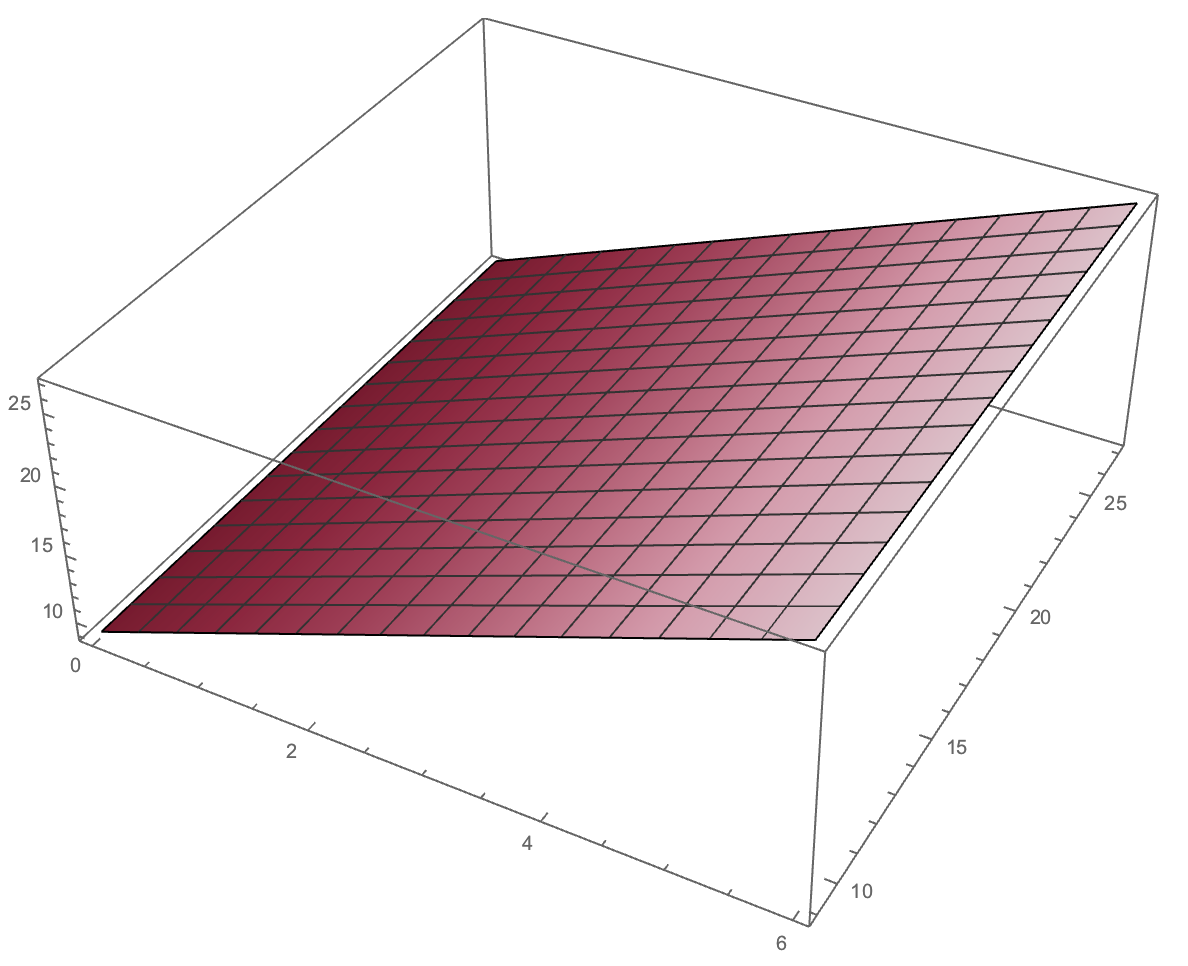
\includegraphics[scale=0.4]{eq_plane.png}
\end{figure}

 A \emph{vector-valued function} or a \emph{vector function} is a function that takes one or more variables (or vectors) as an input and outputs a set of vectors. In other words, the range of a vector-valued function is a set of vectors. For instance, consider the following vector-valued function,
\[
\vec{v}(v_1,v_2) = (v_1,v_2,3)
\]
It takes two scalar inputs ($v_1$ and $v_2$) and returns a vector (i.e. a point) in three-dimensional space. \\

\subsection{The Vector and Parametric Form Equation of a Line}

The mathematical form of a line in $\real^2$ is familiar. We also need a way to represent lines in $\real^n$ where $n>2$. What follows is the mathematical representation of lines in $\real^3$. The extension to $\real^n$ should be intuitive. \\

\begin{framed}
\textbf{Vector and Parametric Form Equation of a Line}
The \emph{vector form equation of a line} is written as $p=t\vec{m}+p_0$, where $p=(x,y,z)$ and $p_0 = (x_0,y_0,z_0)$, $\vec{m} = (a,b,c)$, and $t\in\real$. Expanding this gives,
\[
(x,y,z) = t(a,b,c) + (x_0,y_0,z_0)
\]

The \emph{parametric form equation of the line} $p=t\vec{m}+p_0$ is,
\begin{align*}
x &= ta + x_0 \\
y &= tb + y_0 \\
z &= tc + z_0 
\end{align*}
\end{framed}

So, assuming that we have an initial point $p_0$, some vector $\vec{m}$, and scalar value $t$, we can find any point on the line in three-dimensional space. Typically one might be given two points in $\real^3$ and will be asked to find the equation of the line that connects them. In this case, one of the two points would give us the initial point $p_0$ and the difference between two of these points gives us $\vec{m}$, a line that is parallel to the line that connects the two given points. \\

 The \emph{symmetric equations of a line} are found by solving the parametric equations for $t$ and equating the equations to one another. 
\[
\frac{x-x_0}{a}=\frac{y-y_0}{b}=\frac{z-z_0}{c}
\]
This holds as long as $a,b,c\neq0$.\\

 As an example, say we want to find the equation of the line that passes through points $(2,-1,3)$ and $(1,4,-3)$ in $\real^3$ space. Recall that the difference between two vectors will give you a vector that is parallel to the line that passes through the points that describe those two vectors. Therefore, the vector that is parallel to the line that passes through the points above is,
\[
\vec{m} = (2-1,-1-4,3+3) = (1,-5,6)
\]
Using $\vec{m}$ and some point on the line, say $p_0=(1,4,-3)$, our parametric equations are,
\begin{align*}
x &= t + 1\\
y &= -5t + 4\\
z &= 6t - 3
\end{align*}
which gives us the parametric form equation of a line.\\

The vector form equation of this line is,
\[
(x,y,z) = t(1,-5,6) + (1,4,-3)
\]

\subsection{The Scalar Equation of a Plane}

The equation of a plane requires a bit more work. Let $p_0=(x_0,y_0,z_0)$ be a point on the plane. There exists some vector $\vec{n}=(a,b,c)$ that is orthogonal to the plane. Let $p=(x,y,z)$ be another point on the plane. So we have now defined two points on the plane and a vector orthogonal to the plane. Now let $\vec{r}=p-p_0$. (Recall that $\vec{r}$ will give us a vector that is parallel to the line that connects points $p_0$ and $p$.) We defined $\vec{n}$ to be orthogonal to the plane and $\vec{r}$ as a vector on the plane. Therefore, by definition, $\vec{n}$ is orthogonal to $\vec{r}$, which means the dot product between the two vectors is zero. More formally,
\begin{align*}
\vec{r}\cdot\vec{n} &= 0 \\
(p-p_0)\cdot \vec{n} &=0 \\
(x-x_0,y-y_0,z-z_0) \cdot (a,b,c) &= 0 \\
(x-x_0)a + (y-y_0)b + (z-z_0)c &= 0 
\end{align*}

This is known as the \emph{scalar equation of the plane}. \\
 
\begin{framed}
\textbf{Scalar Equation of the Plane} \\
The scalar equation of the plane is often written as,
\[
ax + by + cz = d
\]
where $d = ax_0 + by_0 + cz_0$. \\
\end{framed}

 As an example, say we want to determine the equation for the plane that contains points $p=(1,-2,0)$, $q=(3,1,4)$, and $r = (0,-1,2)$. Using these points we can find two vectors that sit on this plane,
\begin{align*}
\vec{pq} &= (2,3,4) \\
\vec{pr} &= (-1,1,2) \\
\end{align*}

Now we can find the vector orthogonal to the plane by finding the cross product of the vectors $\vec{pq}$ and $\vec{pr}$. Note that the cross product of two vectors yields a vector that is orthogonal to these vectors. \\

 The cross product can be found by finding the determinant of the following matrix,
\[
\vec{pq}\cdot\vec{pr} 
=
\begin{vmatrix}
\vec{i} & \vec{j} & \vec{k} \\
2 & 3 & 4 \\
-1 & 1 & 2
\end{vmatrix}
=
\vec{i}2-\vec{j}8+\vec{k}5
\]
here, $\vec{i},\vec{j}$, and $\vec{k}$ refer to the standard basis vectors. \\

Using point $p$ and the orthogonal vector $\vec{n}=(2,-8,5)$, the equation for the plane is defined as,
\begin{align*}
2(x-1) - 8(y+2) + 5(z-0) &= 0 \\
2x - 8y + 5z = 18 \\
\end{align*}

To summarize, the steps to finding the equation of a plane in $\mathbb{R}^3$ are outlined below. \\

\begin{framed}
\textbf{Steps to finding the equation of a plane}
\begin{enumerate}
\item Find two vectors on the plane.
\item Using the cross product of the two vectors, find a vector that is orthogonal to the plane.
\item Substitute the orthogonal vector and any point on the plane into the scalar equation of the plane: $a(x-x_0)+b(y-y_0)+c(z-z_0)=0$ where $\vec{n}=(a,b,c)$ is the orthogonal vector and $(x_0,y_0,z_0)$ is a point on the plane. \\
\end{enumerate}
\end{framed}

\pagebreak
\section{Differentiation}

\emph{Differentiation} is the process of computing a derivative. for some arbitrary function $f:\real\rightarrow\real$, the derivative is interpreted as how much $f(x)$ changes as $x$ changes. For example, the slope of a constant function $f(x)$ is found by dividing the change in $f(x)$ by the change in $x$. The slope is the derivative of a single-variable constant function. The definition below generalizes this to all single-variable functions. \\

Consider the function $f:\mathbb{R}\rightarrow\mathbb{R}$. In single variable calculus the derivative of $f(x)$ at the point $x=a$, denoted $df(x)/dx$ or $f'(x)$, is given by evaluating the following limit,
\[
\frac{df(x)}{dx}=\lim_{x\rightarrow a}\frac{f(a)-f(x)}{a-x}
\]

 if we define $a = x + h$ then we can write the derivative as,
\[
\frac{df(x)}{dx}=\lim_{h\rightarrow 0}\frac{f(x+h)-f(x)}{h}
\]

 In vector calculus, instead of having a single equation represent the derivative of a vector valued function $\mathbf{f}$ at point $\vec{a}$ we will have a matrix. This matrix is called the \emph{Jacobian} matrix and represents the total derivative of $\mathbf{f}$ at $\vec{a}$. (Recall that $\mathbf{f}$ is a vector valued function, which means it outputs vectors.\\ 

\subsection{Functions, Graphs, Level Sets, and Vector Fields}

 A \emph{function} \emph{maps} a subset $U$ of $\mathbb{R}^n$ to $\mathbb{R}^m$ if there is a rule $\mathbf{f}$ which associates each vector in $U$ with exactly one vector in $\mathbb{R}^m$. In this context, $U$ is defined as the \emph{domain} of the function $\mathbf{f}$. More formally, we can say that $\mathbf{f}:U\subset\mathbb{R}^n\rightarrow\mathbb{R}^m$. In order to make notation consistent, $\mathbf{f}$ is used when the function represents a map from $\mathbb{R}^n$ to $\mathbb{R}^m$ when $m>1$, and $f$ is used when the function represents a map from $\mathbb{R}^n$ to $\mathbb{R}$. \\
 
 \begin{framed}
 \textbf{The Graph of a Function}\\
  The \emph{graph of a function} $\mathbf{f}:\mathbb{R}^n\rightarrow\mathbb{R}^m$ is the set of points,
 \[
 (x_1, \ldots, x_{n},\ldots,x_{n+m})
 \]
 in $\mathbb{R}^{n+m}$ such that,
 \[
 (x_{n+1},\ldots,x_{n+m}) = \mathbf{f}(x_1, \ldots, x_n)
 \] \\
  \end{framed}
 
 As an example, consider a function $f:U\subset\mathbb{R}\rightarrow\mathbb{R}$ where $f$ is given by,
 \[
 f(x_1) = 3x_1 + 6  
 \]
  The graph of the function would be the set of points $(x_1,x_2)\in\mathbb{R}^2$ such that $(x_2) = f(x_1)$. \\
 
As another example, consider a function $f:U\subset\mathbb{R}^2\rightarrow\mathbb{R}$ where $f$ is given by,
\[
f(x_1,x_2) = x_1^2 + x_2^2
\]
The graph of the function would be the set of points $(x_1,x_2,x_3)\in\mathbb{R}^3$ such that $(x_3) = f(x_1,x_2)$. \\
 
So, if you have n-dimensional inputs and m-dimensional outputs, then the graph of the function that maps the n-dimensional inputs to the m-dimensional outputs will require $m+n$ dimensions. In the examples above, the graph of $f:U\subset\mathbb{R}\rightarrow\mathbb{R}$ requires a two-dimensional space and the graph of $f:U\subset\mathbb{R}^2\rightarrow\mathbb{R}$ requires a three-dimensional space. Similarly, the graph of $f:U\subset\mathbb{R}^2\rightarrow\mathbb{R}^2$ requires a four-dimensional space. \\

\begin{framed}
\textbf{Level Set of a Function} \\
Consider a function $f: U\subset\mathbb{R}^n\rightarrow\mathbb{R}$ and a constant $c\in\mathbb{R}$. Then the \emph{level set of f} is the set of points $(x_1,x_2,\ldots,x_n)\in\mathbb{R}^n$ that satisfy the equation $f(x_1,x_2,\ldots,x_n)=c$. Note that for every value of $c\in\mathbb{R}$ we will have a level set, so if we find the level sets for all values of $c$ then we will obtain a set of level sets. \\
\end{framed}

For instance, consider the function $f:U\subset\mathbb{R}^2\rightarrow\mathbb{R}$ and $z\in\mathbb{R}$. Then the set of points $(x_1,x_2)$ that satisfies the equation $f(x_1,x_2)=z$ is a level set of $f$. In this case, if we find the level sets for all values of $z\in\mathbb{R}$ then we can plot all these level sets. This plot is a contour plot. \\

Below are three examples of a three dimensional plot and the corresponding two dimensional level sets of the function $f:U\subset\real^2\rightarrow \real$. The first example represents the function $f(x,y)=-(x^2+y^2)$. The shape that this function takes on is known as a paraboloid. The second example represents  The third example represents $f(x,y)=\mbox{tanh}(x,y)$, which is also known as the hyperbolic tangent function. \\

\begin{figure}[H]
\centering
\caption{3D and Contour Plot of $f(x,y) = -(x^2+y^2)$}
\label{paraboloid_3d}
\indent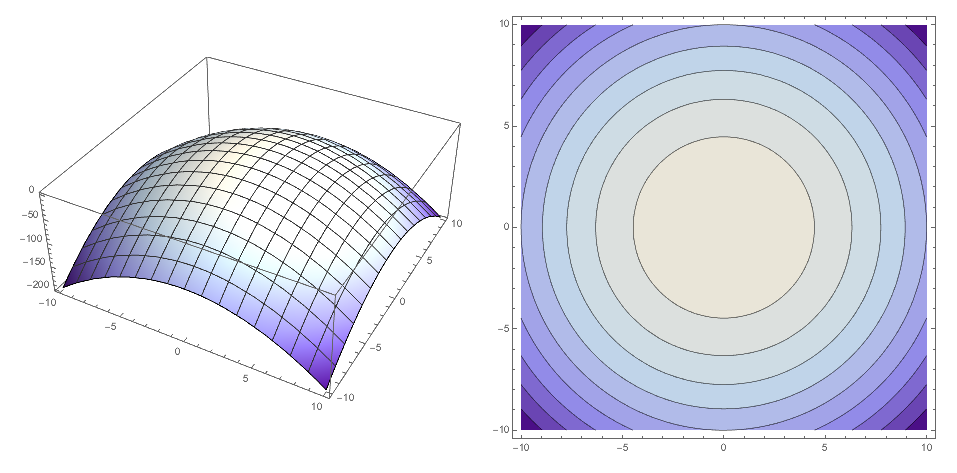
\includegraphics[scale=0.3]{paraboloid_3d.png}
\end{figure}

\begin{figure}[H]
\centering
\caption{3D and Contour Plot of $f(x,y) = \ln(x+y)$}
\label{logarithmic_3d}
\indent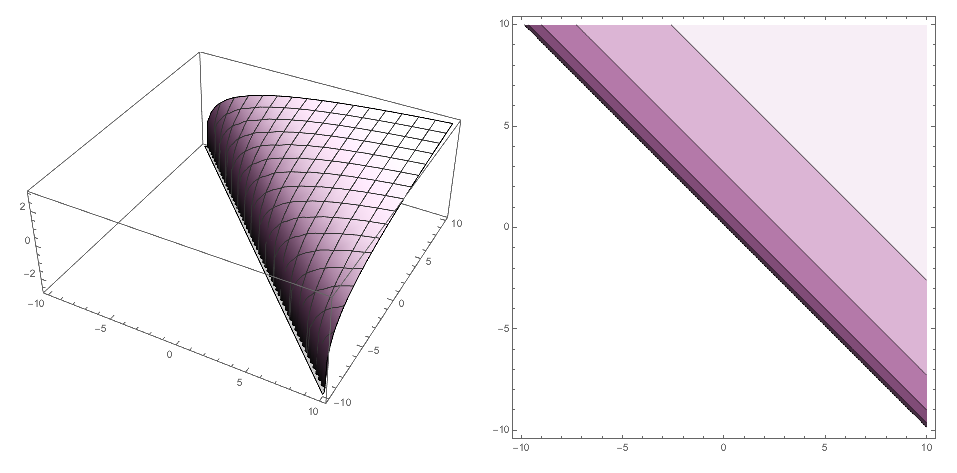
\includegraphics[scale=0.3]{logarithmic_3d.png}
\end{figure}

\begin{figure}[H]
\centering
\caption{3D and Contour Plot of $f(x,y) = \tanh(x-y)$}
\label{hyperbolictangent_3d}
\indent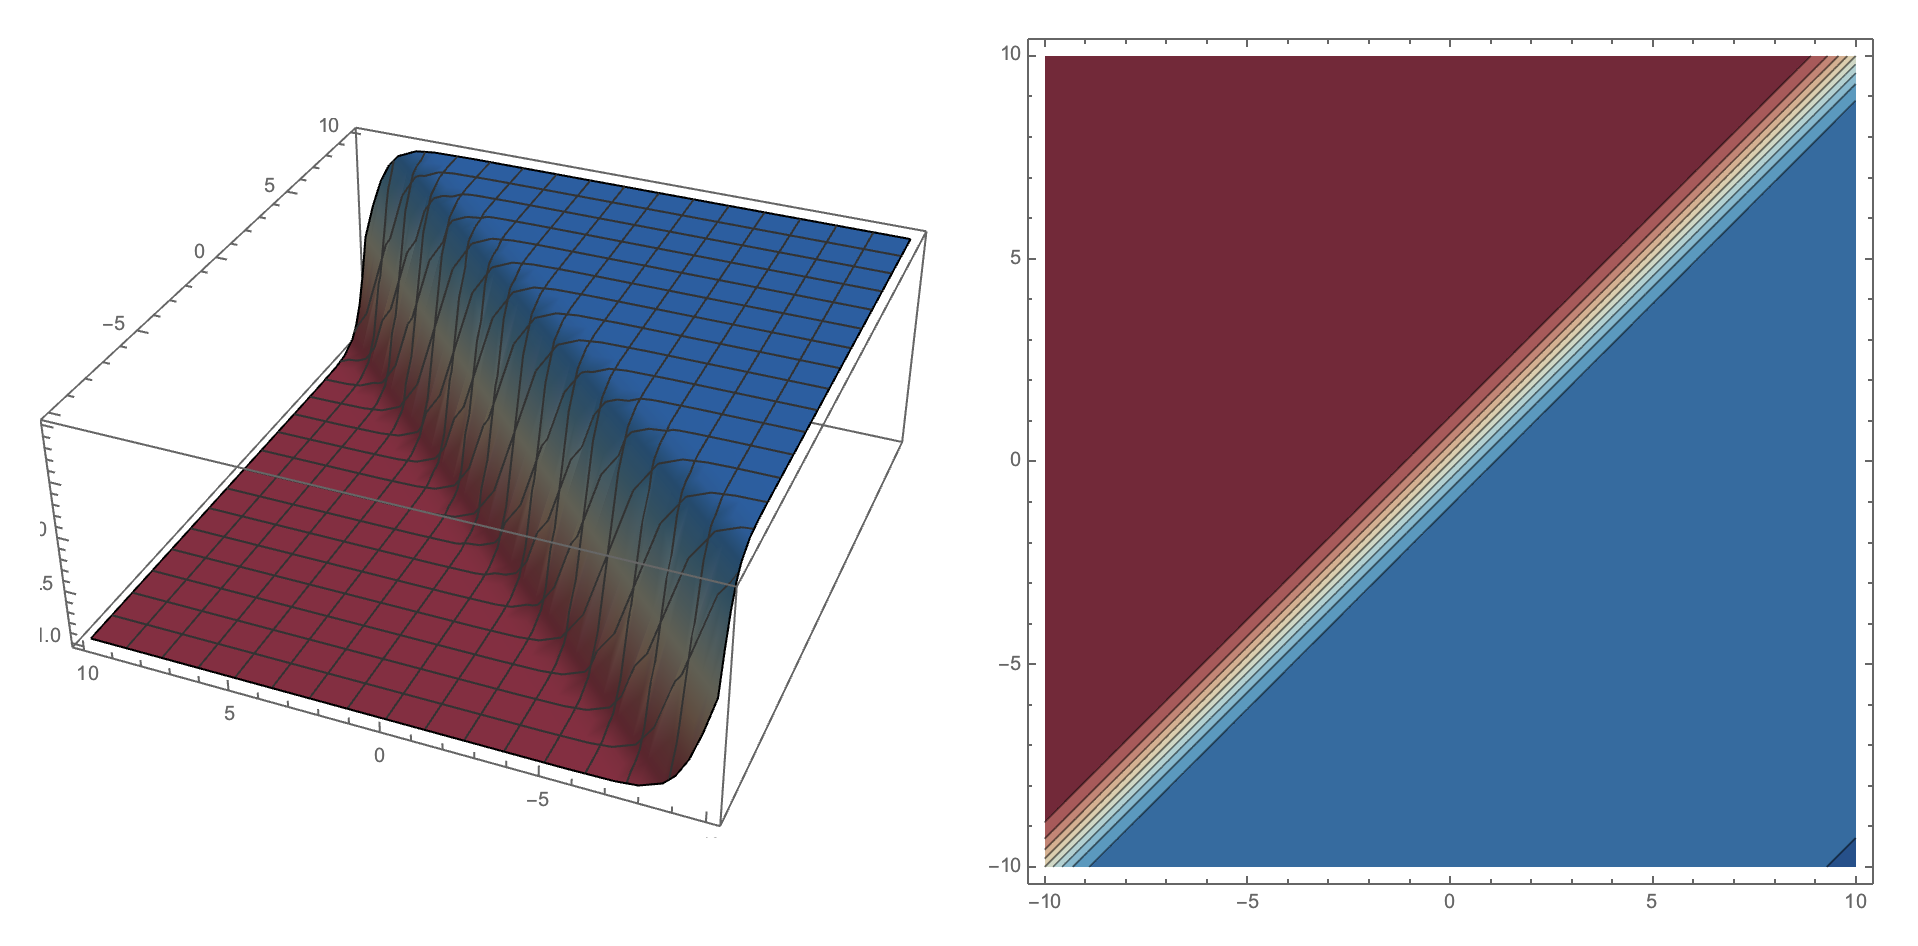
\includegraphics[scale=0.3]{hyperbolictangent_3d.png}
\end{figure}

We can use level sets to examine the correlation between two random variables using, for example, the bivariate normal distribution. The bivariate normal distribution can be plotted in three-dimensions with the x-axis and y-axis representing the two random variables and the z-axis representing the probability density associated with the x-y pair of random variables. Figure~\ref{bivariatenormal} provides an illustration of a pair of uncorrelated and correlated normally distributed variables.\\

\begin{figure}[h]
\centering
\caption{3D and Contour Plots of Bivariate Normal Distributions (Uncorrelated and Correlated)}
\label{bivariatenormal}
\indent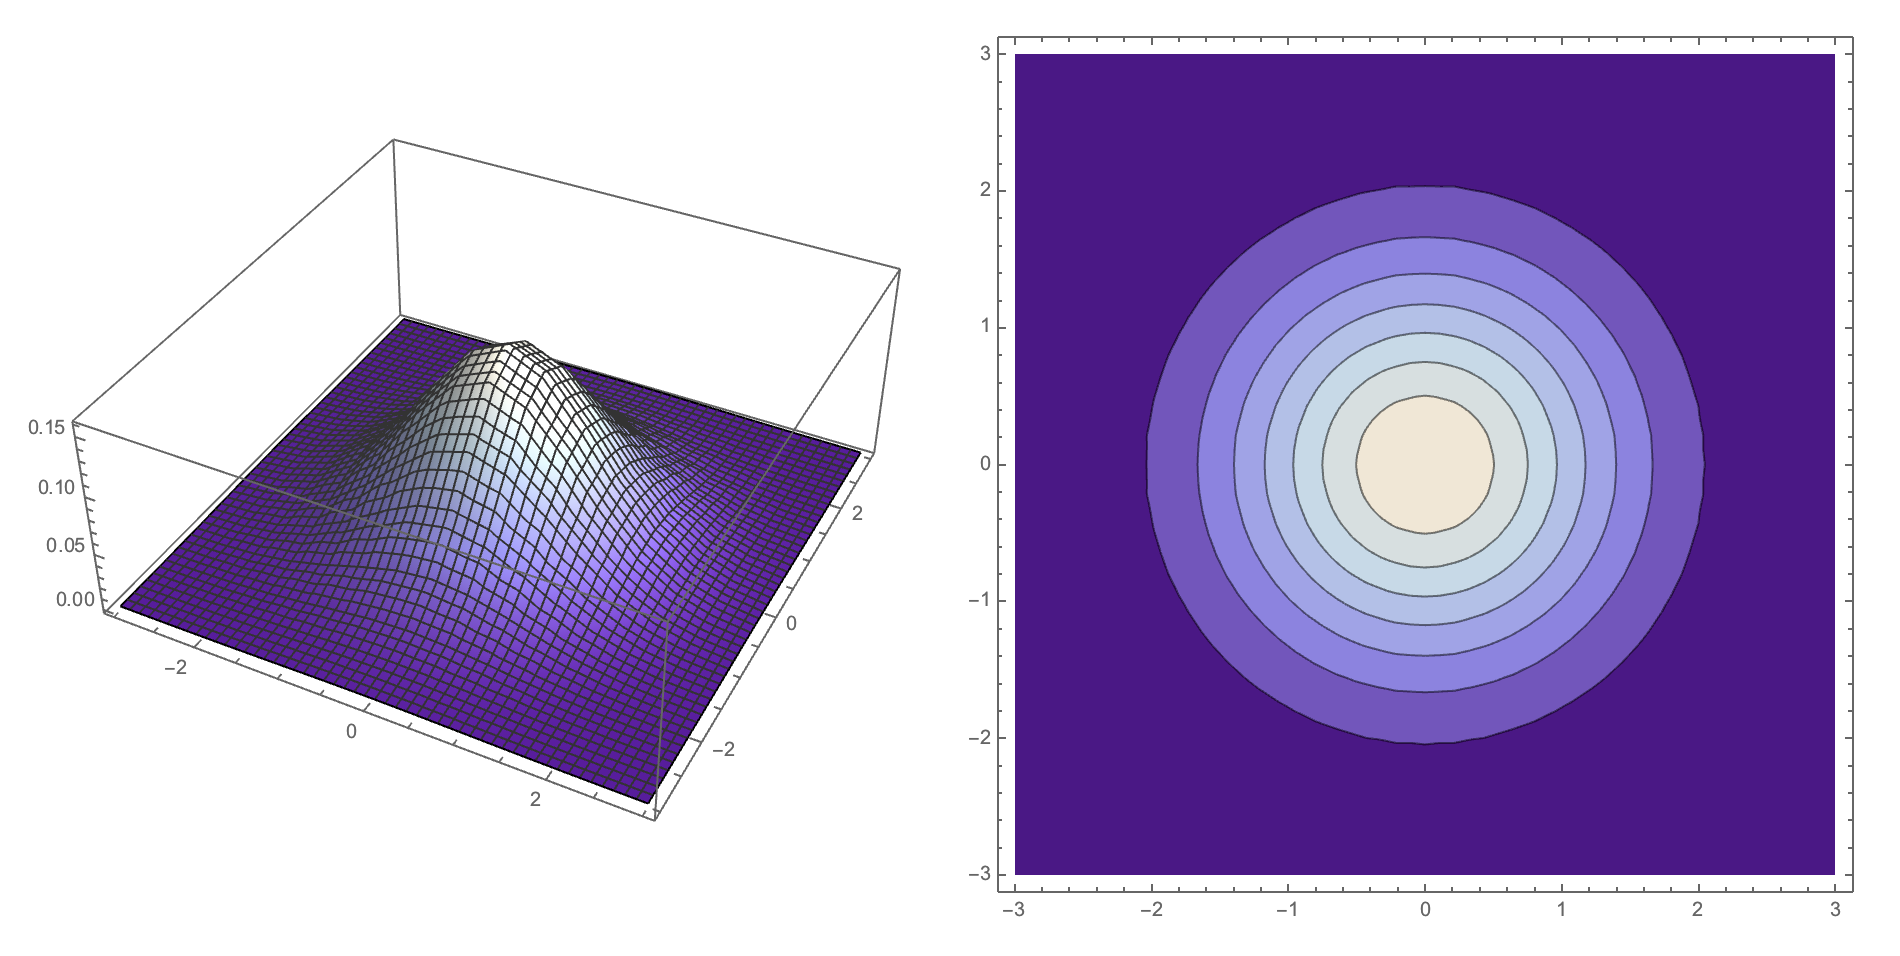
\includegraphics[scale=0.3]{bivariate_3d.png}
\indent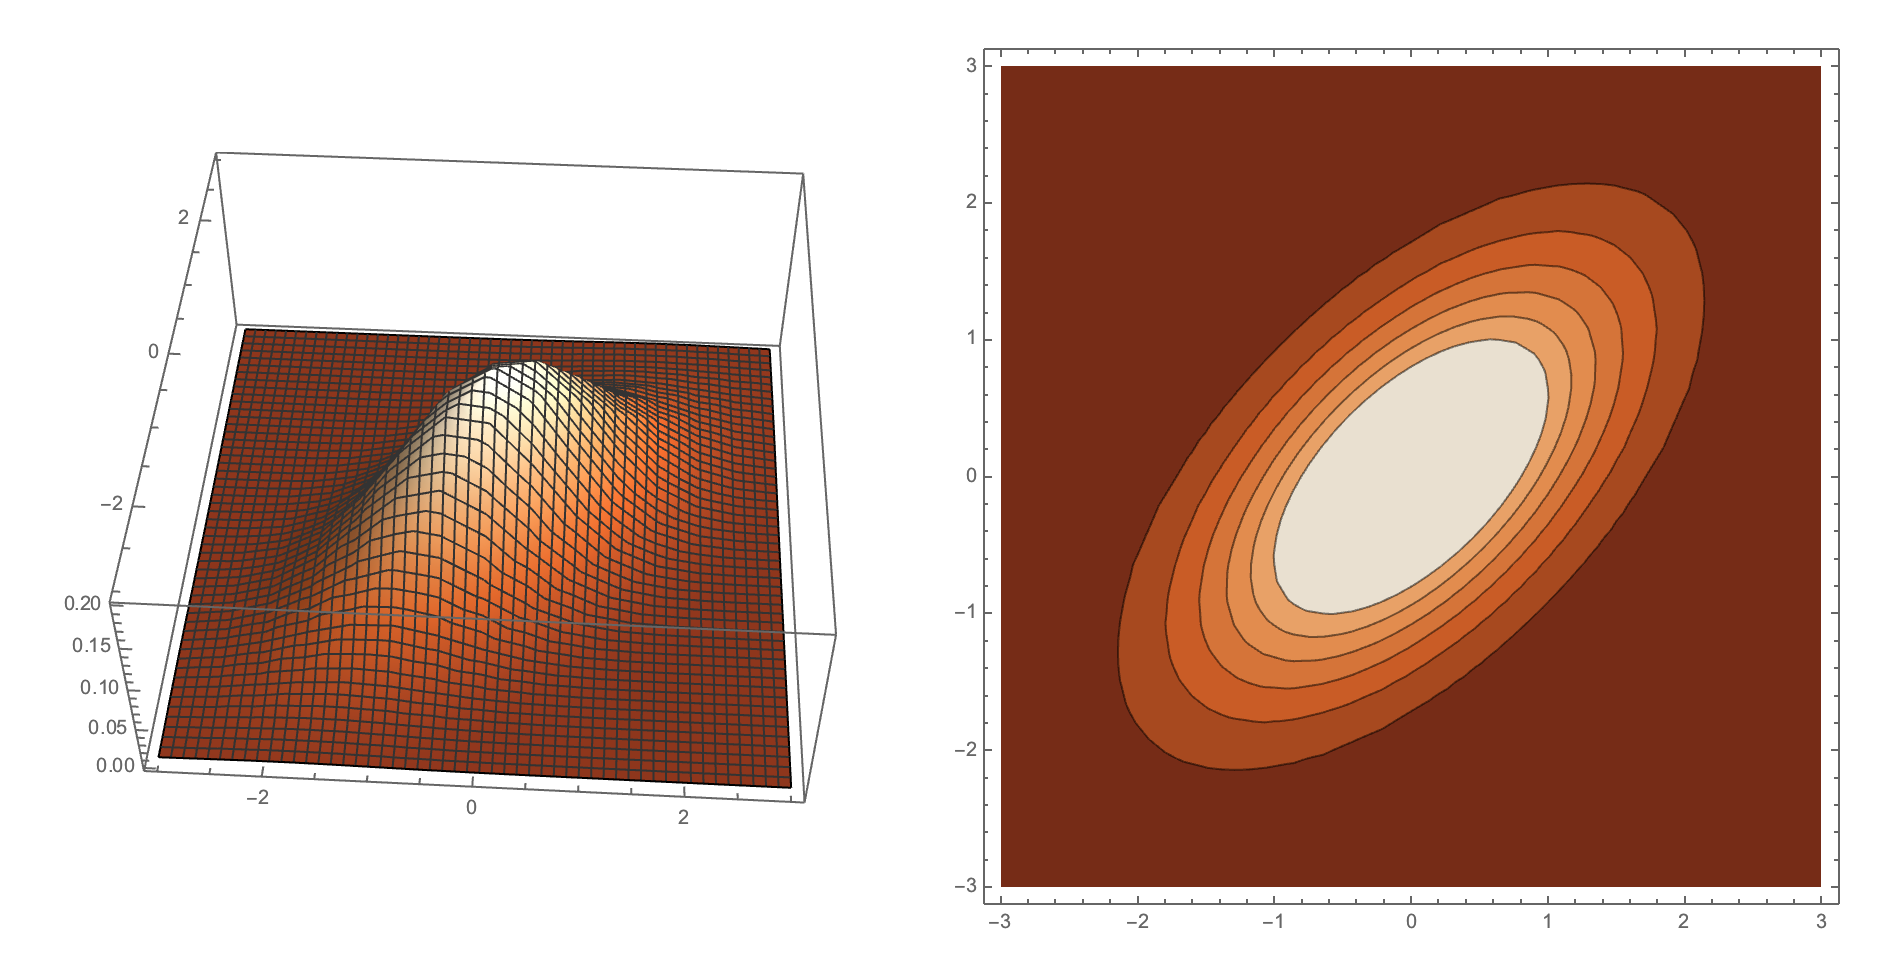
\includegraphics[scale=0.3]{bivariatecorr_3d.png}
\end{figure}

\begin{framed}
\textbf{Vector Field} \\
A \emph{vector field} on $\mathbb{R}^n$ is a function $\mathbf{f}:U\subset\mathbb{R}^n\rightarrow\mathbb{R}^n$. \\ 
\end{framed}

For instance, the function $\mathbf{f}:U\subset\mathbb{R}^3\rightarrow\mathbb{R}^3$ will map three-dimensional vectors into a three-dimensional space. In this case the three-dimensional input vector, $(x,y,z)$, will be the tail of each vector in the vector field and the output $\mathbf{f}(x,y,z)$ will be the head of the vector that starts at $(x,y,z)$. \\

As a two dimensional example $\mathbf{f}:U\subset\mathbb{R}^2\rightarrow\mathbb{R}^2$, Figure~\ref{fig:vectorfield} illustrates the graph of $f(x,y) = (x,y)$ where $-3\leq x,y\leq3$.

\begin{figure}[H]
\centering
\caption{A Vector Field of $f(x,y) = (x,y)$}
\label{fig:vectorfield}
\indent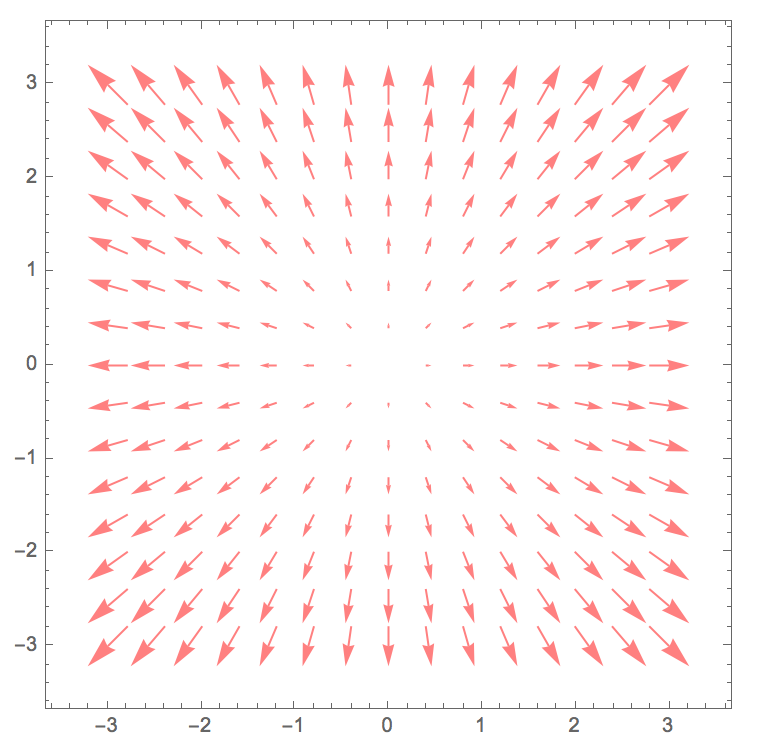
\includegraphics[scale=0.4]{vectorfield.png}
\end{figure}

\subsection{Partial Derivatives}

 If we have a function of several variables, then the each \emph{partial derivative} of this function represents the rate of change of the function with respect to each of the these variables. \\

This can be formally defined using notation similar to the single variable derivative definition. \\

\begin{framed}
\textbf{Partial Derivative} \\
The partial derivative of $f:U\subset\mathbb{R}^n\rightarrow\mathbb{R}$ with respect to $x_i\in\mathbb{R}$ is the function,
\[
\p{f}{x_i}(x_1,x_2,\ldots,x_n) = \lim_{h\rightarrow0}
\frac{f(x_1,\ldots,x_{i-1},x_i+h,x_{i+1},\ldots,x_n) - f(x_1,\ldots,x_{i-1},x_i,x_{i+1},\ldots,x_n)}{h}
\]
\end{framed}

 When applying this definition to a function of several variables we take the partial derivative of the function with respect to $x_i$ by treating all the variables $x_{-i}$ in the function as constants. (The subscript $-i$ refers to every index except $i$.)\\

 Just as with higher-order derivatives in functions of single variables, we also have higher-order derivatives in functions with multiple variables. The \emph{second-order partial derivatives} of a function $f$ with respect to $x_j$ then $x_i$ is defined as,
\[
\frac{\partial^2f}{\partial x_j \partial x_i} = \frac{\partial}{\partial x_j}\frac{\partial f}{\partial x_i}
\]

 When $i\neq j$ we call the partial derivatives \emph{mixed partials}. \\

 Consider two mixed partial derivatives of the same function where in the first case we differentiate with respect to $x_i$ then $x_j$ and in the second case we differentiate with respect to $x_j$ then $x_i$. Then, \emph{Clairaut's Theorem} shows that both of these mixed partial derivatives are equal to one another. \\

\begin{framed}
\textbf{Clairaut's Theorem} \\
Clairaut's Theorem states that if the mixed partials of $f:D\subset\mathbb{R}^2\rightarrow\mathbb{R}$ are defined in an open disk B about a point $\mathbf{a}$ in $D$, and if $\partial^2f/\partial x_j\partial x_i$ and $\partial^2f/\partial x_i\partial x_j$ are continuous at point $\mathbf{a}$ then,
\[
\frac{\partial^2f}{\partial x_j\partial x_i}(\mathbf{a}) = 
\frac{\partial^2f}{\partial x_i\partial x_j}(\mathbf{a})
\]
\end{framed}

\subsection{Differentiation and the Total Derivative}

 A function $\mathbf{f}:U\subset \mathbb{R}^n\rightarrow\mathbb{R}^m$ is \emph{differentiable} at a point $\mathbf{a}\in U$ if there exists a linear transformation $\mathbf{T}:\mathbb{R}^n\rightarrow\mathbb{R}^m$ such that,
\[
\lim_{x\rightarrow a}\frac{|| \mathbf{f(x)}-\mathbf{f(a)}-\mathbf{T(x-a)} ||}{|| \mathbf{x-a} ||}=0
\]
where $\mathbf{T}$ is the \emph{derivative} (or \emph{total derivative}) of \emph{$\mathbf{f}$ at $\mathbf{a}$}.\\

 The total derivative is denoted as $\mathbf{Df(a)}$. So calculating the derivative of the function $\mathbf{f}$ at point $\mathbf{a}$ requires finding the matrix $\mathbf{Df(a)}$. \\

 Formally, we can say that if $f:U\subset\mathbb{R}^n\rightarrow\mathbb{R}$ has partial derivatives that are defined on an open ball about point $\mathbf{a}\in U$ and if the partial derivatives of $f$ with respect to $x_1,x_2,\ldots,x_n$ are continuous at $\mathbf{a}$, then $f$ is differentiable at $\mathbf{a}$ and the derivative of $f$ at $\mathbf{a}$ is given by,
\[
(Df(\mathbf{a}))(\mathbf{x}) = \left[ \p{f}{x_1}\mathbf{a},\p{f}{x_2}\mathbf{a},\ldots, \p{f}{x_n}\mathbf{a} \right]\mathbf{x}
\] 

 In order to find the derivative of a vector valued function at point $\mathbf{a}$ we need the \emph{Jacobian matrix of $f$ at $\mathbf{a}$} denoted $Jf(\mathbf{a})$. \\

\begin{framed}
\textbf{Jacobian Matrix} \\ 
Given the function $f:U\subset\mathbb{R}^n\rightarrow\mathbb{R}$, the Jacobian matrix is,
\[
Jf = \left[ \p{f}{x_1},\p{f}{x_2},\ldots,\p{f}{x_n} \right]
\]
\end{framed}

The extension to a vector valued function $\mathbf{f}:U\subset\real^n\rightarrow\real^m$ should be intuitive. The Jacobian will have $n$ columns and $m$ rows, where each row corresponds to the functions $f_1,f_2,\ldots,f_m$. \\

 As an example, consider the function $f:U\subset\real^2\rightarrow\real$ such that $f(x_1,x_2) = -x_1^2-x_2^2$. The Jacobian of $f(x_1,x_2)$ at any point $\mathbf{a}=(x_1,x_2)$ is given by,
\[
Jf(x_1,x_2) =
\begin{bmatrix}
-2x_1 & -2x_2
\end{bmatrix}
\]
So at any point $\mathbf{a} = (a_1,a_2)$, the derivative of $f(x_1,x_2)$ is given by,
\[
Jf(\mathbf{a}) =
\begin{bmatrix}
-2a_1 & -2a_2
\end{bmatrix}
\begin{bmatrix}
x_1 \\
x_2
\end{bmatrix}
\] \\

 In single variable calculus the linear approximation of a function $f:U\subset\mathbb{R}\rightarrow\mathbb{R}$ at point $a$ where $x\in\mathbb{R}$ is given by,
\[
L(x) = f(x) + f'(x)(x-a)
\]

The extension to a function $f:U\subset\mathbb{R}^n\rightarrow\mathbb{R}$ with multiple input variables is given by,
\[
L(\mathbf{x}) = f(\mathbf{a}) + Jf(\mathbf{a})(\mathbf{x}-\mathbf{a})
\]
The above is the linear approximation of $f(\mathbf{x})$ at point $\mathbf{a}$. \\

 The total derivative of a real-valued function $f:\mathbb{R}^n\rightarrow\mathbb{R}$  can be written using \emph{differential notation},
\[
df = \p{f}{x_1}dx_1 + \p{f}{x_2}dx_2 + \ldots + \p{f}{x_n}dx_n
\]
where $df$ is called the \emph{total differential} of $f$. \\

 Let $\mathbf{f}:U\subset\mathbb{R}^n\rightarrow\mathbb{R}^m$ be given by,
\[
\mathbf{f}(\mathbf{x}) = (f_1(\mathbf{x}),f_2(\mathbf{x}),\ldots,f_m(\mathbf{x}))
\]
The derivative of $\mathbf{f}$ at point $\mathbf{a}$ is the linear transformation $\mathbf{Df(a)}:\mathbb{R}^n\rightarrow\mathbb{R}^m$ given by,
\[
\mathbf{(Df(a))(x)} = 
\begin{bmatrix}
\p{f_1}{x_1}\mathbf{a} & \p{f_1}{x_2}\mathbf{a} & \ldots & \p{f_1}{x_n}\mathbf{a} \\
\p{f_2}{x_1}\mathbf{a} & \p{f_2}{x_2}\mathbf{a} & \ldots & \p{f_2}{x_n}\mathbf{a} \\
\vdots & \vdots & \ddots & \vdots \\
\p{f_m}{x_1}\mathbf{a} & \p{f_m}{x_2}\mathbf{a} & \ldots & \p{f_m}{x_n}\mathbf{a} \\
\end{bmatrix}
\]

From the definition of differentiability we know that,
\[
\mathbf{(f(x)-f(a))-(Df(a)(x-a)}
\]
is approximately 0 for values of $\mathbf{x}$ near $\mathbf{a}$. We can rearrange this to show that,
\[
\mathbf{f(x)\approx f(a) + Df(a)(x-a)}
\]
where $\mathbf{f(a) + Df(a)(x-a)}$ is called the \emph{differential approximation of $\mathbf{f}$ near $\mathbf{a}$}. \\

\subsection{The Chain Rule}

The chain rule in vector calculus is analogous to the chain rule in single variable calculus. If $\mathbf{f}:U\subset\mathbb{R}^m\rightarrow\mathbb{R}^p$ and $\mathbf{g}:\mathbf{f}(U)\rightarrow\mathbb{R}^m$, then the \emph{composition} of $\mathbf{g}$ with $\mathbf{f}$, denoted $\mathbf{g}\circ\mathbf{f}$, is defined by,
\[
(\mathbf{g}\circ\mathbf{f})(\mathbf{x}) = \mathbf{g(f(x))}
\]
This can be thought of as starting with $\mathbf{x}\in\mathbb{R}^m$ and applying the function $\mathbf{f}(\cdot)$, which gives us $\mathbf{f(x)}$. Then we apply the function $\mathbf{g}(\cdot)$ to $\mathbf{f(x)}$, which gives us $\mathbf{g(f(x))}$. \\

\begin{framed}
\textbf{Chain Rule} \\
Let $\mathbf{f}:U\subset\mathbb{R}^n\rightarrow\mathbb{R}^p$ and $\mathbf{g}:\mathbf{f}(U)\rightarrow\mathbb{R}^m$. If $\mathbf{f}$ is differentiable at $\mathbf{a}\in U$ with derivative $\mathbf{Df(a)}$ and $\mathbf{g}$ is differentiable at $\mathbf{f(a)}$ with derivative $\mathbf{Dg(f(a))}$, then the composite function $\mathbf{g}\circ\mathbf{f}$ is differentiable at $\mathbf{a}$ and the derivative of $\mathbf{g}\circ\mathbf{f}$ at $\mathbf{a}$ is the linear transformation $\mathbf{D(g\circ f)(a)}$ given by,
\[
\mathbf{(D(g\circ f)(a))(x) = Dg(f(a))((Df(a))(x)) }
\]
In terms of the Jacobian matrix the derivative of $\mathbf{g\circ f}$ is given by,
\[
J(\mathbf{g\circ f})(\mathbf{a}) = J\mathbf{g(f(a))}J\mathbf{f(a)}
\] 
\end{framed}

 As an example consider two functions $f:U\subset\real^2\rightarrow\real^2$ and $g:f(U)\rightarrow\real^2$. Let, $g(x,y) = (x^2y^3, 3x-y^2)$ and $f(x,y) = (2y, 3x+y^2)$. We are interested in finding the derivative of the composite function $g\circ f$ at $\mathbf{a}=(1,0)$.\\

 The Jacobian for $f(x,y)$ is given by,
\[
Jf(x,y) = 
\begin{bmatrix}
0 & 2 \\
3  & 2y
\end{bmatrix}
\]

 We can substitute $g(w,v)$ into $f(x,y)$ to get the function,
\[
g(f(x,y)) = (4y^2(3x+y^2)^3, 6y-(3x+y^2)^2)
\] 

 The Jacobian for $g(f(x,y))$ is,
\[
Jg(f(x,y)) = 
\begin{bmatrix}
36y^2(3x+y^2)^2 & 24y^3(3x+y^2)^2 + 8y(3x+y^2)^3 \\
-6(3x+y^2) & 6 - 4y(3x+y^2) \\
\end{bmatrix}
\]

 The Jacobians $Jg(f(x,y))$ and $Jf(x,y)$ evaluated at $\mathbf{a}$ are,
\[
Jg(f(\mathbf{a})) = 
\begin{bmatrix}
0 & 0 \\
-18 & 6
\end{bmatrix}
,
Jf(\mathbf{a}) = 
\begin{bmatrix}
0 & 2 \\
3 & 0
\end{bmatrix}
\]

 Finally, the derivative of $g\circ f$ at point $\mathbf{a}$ is,
\[
Jg(f(\mathbf{a}))Jf(\mathbf{a}) = 
\begin{bmatrix}
0 & 0 \\
-18 & 6
\end{bmatrix}
\begin{bmatrix}
0 & 2 \\
3 & 0
\end{bmatrix}
=
\begin{bmatrix}
0 & 0 \\
18 & -36
\end{bmatrix}
\]

To summarize, the chain rule applied to a vector valued function nested in another vector valued function is just the product of the Jacobian of the outer function evaluated at the inner function and the Jacobian of the inner function. This can be easily extended to multiple nested functions. \\ 

\pagebreak

\section{Applications of Differentiation}

\subsection{Gradient, Divergence, and Curl}

The gradient is the Jacobian of a function that goes from $\real^n$ to $\real$. \\

\begin{framed}
\textbf{Gradient} \\
The \emph{gradient} of $f:U\subset\mathbb{R}^n\rightarrow\mathbb{R}$ is the vector-valued function,
\[
\nabla f(\mathbf{x}) = \left( \p{f}{x_1}(\mathbf{x}), \p{f}{x_2}(\mathbf{x}), \ldots, \p{f}{x_n}(\mathbf{x}) \right)
\]
\end{framed}

 For example, consider the function $f:U\subset\mathbb{R}^3\rightarrow\mathbb{R}$ where $f(\mathbf{x}) = x_1^2x_2^2 + 2x_1 + 3x_3^3x_1$. Then the gradient of $f(\mathbf{x})$ is, 
\[
\nabla f(\mathbf{x}) = (2x_1x_2^2 + 2 + 3x_3^3, 2x_1^2x_2, 9x_3^2x_1)
\] \\

The directional derivative represents the rate of change of the function at point $\mathbf{a}$ in the direction of $\mathbf{u}$. Recall that a unit vector is a vector with length 1 and $\hat{\mathbf{u}} = \frac{\mathbf{u}}{||\mathbf{u}||}$ is the unit vector in the direction of $\mathbf{u}$. \\

\begin{framed}
\textbf{Directional Derivative} \\
Let $f:U\subset\mathbb{R}^n\rightarrow\mathbb{R}$, let $\mathbf{a}\in U$, and let $\mathbf{u}$ be the unit vector in $\mathbb{R}^n$. The \emph{directional derivative} of $f$ \emph{at $\mathbf{a}$ in the direction $\mathbf{u}$} is,
\[
D_{\mathbf{u}}f(\mathbf{a}) = \lim_{h\rightarrow0} \frac{f(\mathbf{a}+h\mathbf{u})-f(\mathbf{a})}{h}
\] 

So if $f:U\subset\mathbb{R}^n\rightarrow\mathbb{R}$ is differentiable at $\mathbf{a}$ and $\mathbf{u}$ is a unit vector then the directional derivative $D_{\mathbf{u}}f(\mathbf{a})$ exists and,
\[
D_{\mathbf{u}}f(\mathbf{a}) = \nabla f(\mathbf{a})\cdot\mathbf{u} 
\]
\end{framed} 

As an example, consider the function $f(x_1,x_2) = 3x_1^2x_2 + x_2^2x_1^2$. To find the directional derivative $f(x_1,x_2)$ at the point $(-1,1)$ in the direction $(4,8)$ we first find the gradient,
\[
\nabla f(x_1,x_2) =  (6x_1x_2 + 2x_2^2x_1, 3x_1^2+2x_2x_1^2)
\]
We can define $\mathbf{a}=(-1,1)$ and $\mathbf{u}=(4,8)$. A unit vector in the prescribed direction is,
\[
\mathbf{u} = \frac{(4,8)}{\sqrt{16+64}} = \frac{(4,8)}{\sqrt{80}}
\]
Then we have,
\[
D_{\mathbf{u}}f(\mathbf{a}) \cdot \mathbf{u} =  (-8,5) \cdot \frac{(4,8)}{\sqrt{80}} = \frac{8}{\sqrt{80}}
\]
so the directional derivative of the function at $(-1,1)$ in the direction $(4,8)$ is $\frac{8}{\sqrt{80}}$. \\

 If $\nabla f(\mathbf{a})\neq\mathbf{0}$ and the level curve of $f$ through $\mathbf{a}$ has a tangent vector $\mathbf{t}$ at $\mathbf{a}$, then $\nabla f(\mathbf{a})$ is perpendicular to $\mathbf{t}$. We can show this by considering the function $f:U\subset\real^2\rightarrow\real$. Let $\mathbf{a},\mathbf{x}\in\real^2$ and $f(x_1,x_2)=c$ be the equation for the level curve of $f$ through $\mathbf{a}$. Parameterize the level curve by $\mathbf{x}=\mathbf{r}(t)$ where $\mathbf{r}(0)=\mathbf{a}$. We can substitute $\mathbf{r}(t)$ into f, which gives,
\[
f(\mathbf{r}(t)) = c
\]
Differentiating the equation gives,
\[
\nabla f(\mathbf{r}(t))\cdot\mathbf{r}'(t) = 0
\]
By definition when $t=0$,
\[
\nabla f(\mathbf{a})\cdot\mathbf{r}'(0) = 0
\]
Recall that two vectors are perpendicular if they are orthogonal (i.e. their dot product equals 0). Also recall that $\mathbf{r}'(0)$ is the tangent vector to the level curve at $\mathbf{a}$. It follows that if $\mathbf{r}'(0)\neq\mathbf{0}$, then $\nabla f(\mathbf{a})$ is perpendicular to the to the vector that is tangent to the level curve at $\mathbf{a}$. \\

A geometric interpretation of the gradient of a function is that it points in the direction of the largest increase of the function. Since $\nabla f(\mathbf{a})$ points in the direction of the largest increase in $f$, and if we have two level curves where $c_2>c_1$, then $\nabla f(\mathbf{a})$ will point to $f(x_1,x_2) = c_2$. \\

 These concepts can be extended to higher dimensions. For instance, given the function $f:U\subset\real^3\rightarrow\real$, we will have a level surface (instead of a level curve) and the gradient of $f$ at $\mathbf{a}\in\real^3$ is perpendicular to a plane (instead of a vector) that is tangent to the level surface at $\mathbf{a}$. Note that there exists a bundle of tangent vectors at $\mathbf{a}$ that are each perpendicular to the gradient of $f$. \\

To summarize, the gradient of a function at some point $\mathbf{a}$ gives the direction of the greatest increase from point $\mathbf{a}$. It follows that the negative of the gradient will give the direction of the greatest decrease. (Note, moving perpendicular to the gradient will give no change.) The directional derivative is the dot product of the gradient and some specified direction from point $a$ and will give you the rate of change of moving in that direction. \\

Previously we introduced the concept of a vector field. In addition to the total derivative of a vector field, we can specify the divergence and curl of a vector field. \\

\begin{framed}
\textbf{Divergence and Curl} \\
Consider the differentiable vector field $\mathbf{F}:U\subset\real^3\rightarrow\real^3$. Also, let $\nabla$ represent the vector $(\p{}{x},\p{}{y},\p{}{z})$ \\

 The \emph{divergence} of $\mathbf{F}$ is the dot product,
\[
\mbox{div}(\mathbf{F}) = \nabla\cdot\mathbf{F}
\]
and the \emph{curl} of $\mathbf{F}$ is the cross product,
\[
\mbox{curl}(\mathbf{F}) = \nabla\times\mathbf{F}
\]
\end{framed}

Note that $\mbox{div}(\mathbf{F})$ is a scalar-valued function and $\mbox{curl}(\mathbf{F})$ is a vector field. Also note that $\mbox{div}(\mathbf{F})$ is simply the trace of the Jacobian of $\mathbf{F}$. \\

As an example, consider the vector field $\mathbf{F}:U\subset\real^3\rightarrow\real^3$ where $\mathbf{F}(x,y,z)=(3xy, x^2yz^3, 2y^2z)$. Then we have,
\[
\mbox{div}({\mathbf{F}}) = 3y + x^2z^3 + 2y^2
\]
and,
\begin{align*}
\mbox{curl}(\mathbf{F}) &= 
\begin{vmatrix}
\mathbf{i} & \mathbf{j} & \mathbf{k} \\
\p{}{x} & \p{}{y} & \p{}{z} \\
3xy & x^2yz^3 & 2y^2z 
\end{vmatrix} \\
&= (4yz - 3x^2yz^2)\mathbf{i} + (2xyz^3 - 3x)\mathbf{k} \\
&= (4yz - 3x^2yz^2, 0, 2xyz^3 - 3x)
\end{align*}

\subsection{The Hessian Matrix}

Just like the Jacobian is the matrix of first-order derivatives, the Hessian is the matrix of second-order derivatives. \\

\begin{framed}
\textbf{Hessian Matrix} \\
Consider the function $f:U\subset\real^n\rightarrow\real$ that has second-order partials at $\mathbf{a}\in U$. The \emph{Hessian matrix} for $f$ at $\mathbf{a}$ is,
\[
Hf(\mathbf{a}) = \left[ \p{^2f}{x_j\partial x_i} \right] (\mathbf{a})
\]

The \emph{Hessian form for $f$ at $\mathbf{a}$} is the quadratic form defined by,
\[
h(\mathbf{x}) = \mathbf{x}^\top Hf(\mathbf{a})\mathbf{x}
\]
\end{framed}

For a function of several variables, the Hessian is analogous to the second derivative of single variable function. The Hessian represents the second derivative of a function at point $\mathbf{a}$. We can also say that the Hessian matrix is the Jacobian matrix of the gradient of a function. More formally,
\[
Hf(\mathbf{x}) = J\nabla f(\mathbf{x})
\]

 As an example, consider the function $f:U\subset\real^2\rightarrow\real$ where $f(x,y) = 3x^2 + e^{2y} +xy^3$. The Hessian matrix of $f(x,y)$ for any $\mathbf{a}\in\real^2$ is,
\[
Hf(\mathbf{a}) = 
\begin{bmatrix}
6 & 3y^2 \\
3y^2 & 4e^{2y}+6xy  \\
\end{bmatrix}
(\mathbf{a})
\]

 The Hessian form is 
\[
h(x,y) = 
\begin{bmatrix}
x & y \\
\end{bmatrix}
\begin{bmatrix}
6 & 3y^2 \\
3y^2 & 4e^{2y}+6xy  \\
\end{bmatrix}
(\mathbf{a})
\begin{bmatrix}
x \\
y \\
\end{bmatrix}
\]

 At the point $(-3,2)$ the Hessian matrix is,
\[
Hf(-3,2) = 
\begin{bmatrix}
6 & 12 \\
12 & 4e^{4}-36  \\
\end{bmatrix}
\]
and the Hessian form is,
\begin{align*}
h(x,y) &= 
\begin{bmatrix}
x & y \\
\end{bmatrix}
\begin{bmatrix}
6 & 12 \\
12 & 4e^{4}-36  \\
\end{bmatrix}
\begin{bmatrix}
x \\
y \\
\end{bmatrix} \\
&= 
\begin{bmatrix}
x & y \\
\end{bmatrix}
\begin{bmatrix}
6x + 12y \\
12x + (4e^{4}-36)y  \\
\end{bmatrix} \\
&=
6x^2 + 24xy +  (4e^{4}-36)y^2
\end{align*}

\subsection{Local Extrema}

 Just like with single variable calculus, we are interested in the points that achieve a maximum or minimum of some function. In single variable calculus we are given some function $f:U\subset\real\rightarrow\real$. If $f'(a)=0$ and $f''(a)>0$ then $f(a)$ is a local minimum. If $f'(a)=0$ and $f''(a)<0$ then $f(a)$ is a local maximum. \\

 Similarly, for functions of several variables $f:U\subset\real^n\rightarrow\real$, if $\grad f(\mathbf{a})=\mathbf{0}$ then \emph{a negative definite Hessian matrix means that $f(\mathbf{a})$ is a local maximum and a positive definite Hessian matrix means that $f(\mathbf{a})$ is a local minimum}. An \emph{indefinite Hessian matrix means that $f(\mathbf{a})$ is a saddle point}. If a local extremum exists at point $\mathbf{a}$ then either $\grad f(\mathbf{a})=\mathbf{0}$ or the gradient of $f$ is undefined at point $\mathbf{a}$. In this context, the point $\mathbf{a}$ is defined as a \emph{critical point}.  \\

 The maximum/minimum values of functions of several variables require and understanding of positive/negative definiteness of the Hessian matrix. Let $\mathbf{M}$ be some real matrix and let $\mathbf{x}$ be a non-zero vector of real numbers. Then $\mathbf{M}$ is a positive definite matrix if the scalar $\mathbf{x}^\top\mathbf{M}\mathbf{x}$ is positive for every vector $\mathbf{x}$. Similarly, $\mathbf{M}$ is a negative definite matrix if the scalar $\mathbf{x}^\top\mathbf{M}\mathbf{x}$ is negative for every vector $\mathbf{x}$. \\

 Just like in single variable calculus, we can specify a second derivative test for functions $f:U\subset\real^n\rightarrow\real$. Let $\mathbf{a}\in U$ and $\grad f(\mathbf{a})=\mathbf{0}$. We can define submatrices $H_1,H_2,\ldots,H_n$ of the Hessian matrix $Hf(\mathbf{a})$ as follows,
\[
H_1 = 
\begin{bmatrix}
h_{11}
\end{bmatrix},
H_2 = 
\begin{bmatrix}
h_{11} & h_{12} \\
h_{21} & h_{22}
\end{bmatrix},
\ldots,
H_n = 
\begin{bmatrix}
h_{11} & \ldots & h_{1n} \\
\vdots & \ddots & \vdots \\
h_{n1} & \ldots & h_{nn}
\end{bmatrix}
\] 
We can apply these ``subhessian matrices'' to find local extrema.

\begin{framed}
\textbf{Local Extrema Rules}
\begin{itemize}
\item $f$ has a local minimum at $\mathbf{a}$ if,
\[
|H_1| >0, |H_2| >0, \ldots, |H_n| >0
\]
\item $f$ has a local maximum at $\mathbf{a}$ if,
\[
|H_1| <0, |H_2| >0, |H_3| <0, |H_4| >0, \ldots
\]
\item $f$ has a saddle point at $\mathbf{a}$ if $|H_i|\neq0$ for $i=1,\ldots,n$ and the signs of the determinants do not follow the patterns for a minimum or maximum (defined above). 
\item There is no information about $f$ at point $\mathbf{a}$ being a local extrema if $|H_i|=0$ for any $i=1,\ldots,n$.
\end{itemize}
\end{framed}

 As an example consider the function $f:U\subset\real^2\rightarrow\real$ where $f(x,y) = x^2 + y^2$. To find the local extrema of this function we have to find the Hessian matrix. The Jacobian matrix is,
\[
Jf(x,y) = \grad f(x,y) =
\begin{bmatrix}
 2x \\
 2y                                           
\end{bmatrix}
\]
 The Hessian matrix is,
\[
Hf(x,y) = 
\begin{bmatrix}
2 & 0 \\
0 & 2
\end{bmatrix}
\]
It follows that $|H_1|=2>0$ and $|H_2|=4>0$, and the critical point $\mathbf{a}=(0,0)$ is where the function reaches a minimum. \\

\subsection{Constrained Optimization}

Constrained optimization deals with finding solutions to an ``objective'' equation given some ``constraint'' equation. The purpose is to find the extrema of the objective function while satisfying the constraint. \\

Consider the functions $f:U\subset\real^n\rightarrow\real$ and $g:U\real^n\rightarrow\real$. Let $\mathbf{a}$ and $\lambda^*$ be solutions to the following system of equations,
\begin{align*}
\grad f(\mathbf{x}) &= \lambda\grad g(\mathbf{x}) \\
g(\mathbf{x}) &= 0
\end{align*}
Also, let $W(\mathbf{x},\lambda) = Hf(\mathbf{x})-\lambda Hg(\mathbf{x})$. If $W(\mathbf{a},\lambda^*)$ is positive definite, then $f(\mathbf{a})$ is a local minimum value of $f$ along $g(\mathbf{x}) = 0$. $W(\mathbf{a},\lambda^*)$ is negative definite, then $f(\mathbf{a})$ is a local maximum value of $f$ along $g(\mathbf{x}) = 0$.

The remainder of this section deals with the application of constrained optimization to information theory. In information theory, entropy (specifically Shannon Entropy) is a measure of the disorder or uncertainty of information content. It is defined as,
\[
E[I(X)] = -\sum_{i=1}^{n} P(x_i)\ln P(x_i)
\]
where $P(x_i)$ refers to the probability of the random variable $x_i$.  \\

 Therefore, our constrained optimization problem is the following,
\begin{align*}
& \max\ E[I(X)] \\
& \mbox{where } \sum_{i}^{n} P(x_i) = 1
\end{align*}

 The gradients we need to find are,
\[
\grad E[I(X)] = 
-
\begin{bmatrix}
\ln P(x_1) + 1 \\
\ln P(x_2) + 1 \\
\vdots \\
\ln P(x_n)  + 1
\end{bmatrix}
\]
and,
\[
\grad \lambda \left( \sum_{i}^{n} P(x_i) -1 \right) = 
\lambda
\begin{bmatrix}
1 \\
1 \\
\vdots \\
1
\end{bmatrix}
\]
This gives us the following system of equations,
\begin{align*}
-\ln P(x_1) + 1 &= \lambda \\
-\ln P(x_1) + 1 &= \lambda \\
\vdots \\
-\ln P(x_1) + 1 &= \lambda \\
\sum_{i}^{n} P(x_i) = 1
\end{align*}
So we have $n+1$ unknowns and $n+1$ equations. All but the last equation gives,
\[
P(x_1) = P(x_2) = \ldots = P(x_n) = e^{1-\lambda}
\]
We can substitute this into the last equation and solve for $\lambda$,
\begin{align*}
ne^{1-\lambda} &= 1 \\
e^{1-\lambda} &= \frac{1}{n} \\
1-\lambda &= \ln \left(\frac{1}{n}\right) \\
\lambda &= 1 - \ln \left(\frac{1}{n} \right)
\end{align*}
Putting this result into $e^{1-\lambda}$ gives,
\[
P(x_1)=P(x_2)=\ldots=P(x_n)=\frac{1}{n}
\]

 In order to find if this is the maximum of $E[I(X)]$ we need to evaluate the difference in Hessians, $W(\frac{1}{n},\lambda^*)$. So we have,
\[
HE[I(X)] = 
\begin{bmatrix}
- \frac{1}{P(x_1)} & 0 & \ldots & 0 \\
0 & - \frac{1}{P(x_2)} & \ldots & 0 \\
\vdots & \ddots & \ddots & \vdots \\
0 & 0 & \dots & - \frac{1}{P(x_n)} 
\end{bmatrix}
\]
and,
\[
\lambda H\left(\sum_{i}^{n} P(x_i)-1\right) = \lambda \mathbf{0}_{n\times n}
\]
It follows that,
\[
W\left(\frac{1}{n},\lambda^*\right) = HE[I(X)] - H\left(\sum_{i}^{n} P(x_i)-1\right) = 
\begin{bmatrix}
- \frac{1}{P(x_1)} & 0 & \ldots & 0 \\
0 & - \frac{1}{P(x_2)} & \ldots & 0 \\
\vdots & \ddots & \ddots & \vdots \\
0 & 0 & \dots & - \frac{1}{P(x_n)} 
\end{bmatrix}
=
\begin{bmatrix}
- n & 0 & \ldots & 0 \\
0 & - n & \ldots & 0 \\
\vdots & \ddots & \ddots & \vdots \\
0 & 0 & \dots & - n 
\end{bmatrix}
\]
This matrix is negative definite. So the values of $P(x_i)= \frac{1}{n}$ maximize entropy. The maximum value of entropy is,
\[
E[I(X)] = -\sum_{i=1}^{n} \frac{1}{n} \ln \left(\frac{1}{n}\right) =  - \ln\left(\frac{1}{n}\right) = -( \ln 1 - \ln n ) = \ln n
\]

 A two-sided coin, for example, can produce a maximum entropy of $\ln(2)\approx 0.693$. On the other hand a coin that is heads on both sides produces an entropy of $\ln(1)=0$. In other words, the coin with heads on both sides can be predicted with certainty so the entropy (i.e. measure of unpredictability) is zero. Since we are using the natural logarithm (logarithm with base $e$) the measurement of entropy is in nats. So the numbers 0-9 produce approximately 2.30 nats. \\
 
\pagebreak
\section{Integration}

\subsection{Paths and Arclength}

A \emph{path} is a continuous vector valued function $\mathbf{f}$ from $\real$ to $\real^n$. There are different types of paths. Define a path as $\mathbf{f}:[a,b]\rightarrow\real^n$. This means that $\mathbf{f}(t_1)\neq\mathbf{f}(t_2)$ for all $t_1$ and $t_2$ in (a,b) such that $t_1\neq t_2$. A path is simple if it has no points of self-intersection except possibly at the end points. A path is closed if $\mathbf{f}(b)=\mathbf{f}(a)$. A path is smooth if $\mathbf{f}'(t)$ is continuous and $\mathbf{f}'(t)\neq\mathbf{0}$. A path is piecewise smooth if there are finitely many subintervals of [a,b] on which the path is smooth. Note that a path is a function and the curve is the image $\mathbf{f}(I)$, where $I=[a,b]$, of the path function.\\

Formally, a \emph{curve} or \emph{arc} is a set of points $\mathbf{f}(I)$ such that $\mathbf{f}:I\rightarrow\real^n$, where $I=[a,b]$. Here, $\mathbf{f}(I)$ is the \emph{image} of the path function. \\

\begin{framed}
\textbf{Path Length and Arclength} \\
The \emph{length} or \emph{arclength} of a simple smooth path $\mathbf{f}(t)$ where $a\leq t \leq b$ is defined as,
\[
\int_a^b || \mathbf{f}'(t) || dt
\]
\end{framed}

In words this is just the integral of the magnitude of the Jacobian of the vector valued path function $\mathbf{f}(t)$. \\

The physical interpretation of this is that the derivative of a vector valued path function gives the velocity vector. Velocity has two components: direction and magnitude. The magnitude component is equivalent to the concept of speed in physics. Thus, path length is the integral of speed, over the time interval $a$ to $b$. \\ 

Consider the typical parametrized function that defines a unit circle, $\mathbf{f}(t) = (\cos{t},\sin{t})$. Figure~\ref{fig:arclengthcircle} provides an illustration of the unit circle. One revolution around the circumference of a circle corresponds to the variable $t$ going from $0$ to $2\pi$. (Recall, this comes from the definition of $\pi$ being equal to the ratio of the circumference to the diameter, which implies that $2\pi r$ is equal to the circumference of a circle with radius $r$.) We can convince ourselves that the definition of path length is correct by evaluating two revolutions of the circle, we know to be equal to $4\pi\approx 12.57$. First find the gradient,
\[
\mathbf{f}'(t) = (-\sin{t}, \cos{t})
\]
Now find the magnitude of the gradient,
\[
\norm{\mathbf{f}'(t)} = \sqrt{\sin{^2t} + \cos{^2t}} = \sqrt{1} = 1
\]
Now find the definite integral,
\[
\int_{0}^{4\pi} \norm{\mathbf{f}'(t)} \ dt = \int_{0}^{4\pi} 1 \ dt = [t]_{0}^{4\pi} = 4\pi
\]

\begin{figure}[h]
\centering
\caption{Plot of $\mathbf{f}(t) = (\cos{t}, \sin{t})$ where $0\leq t\leq 4\pi$}
\label{fig:arclengthcircle}
\indent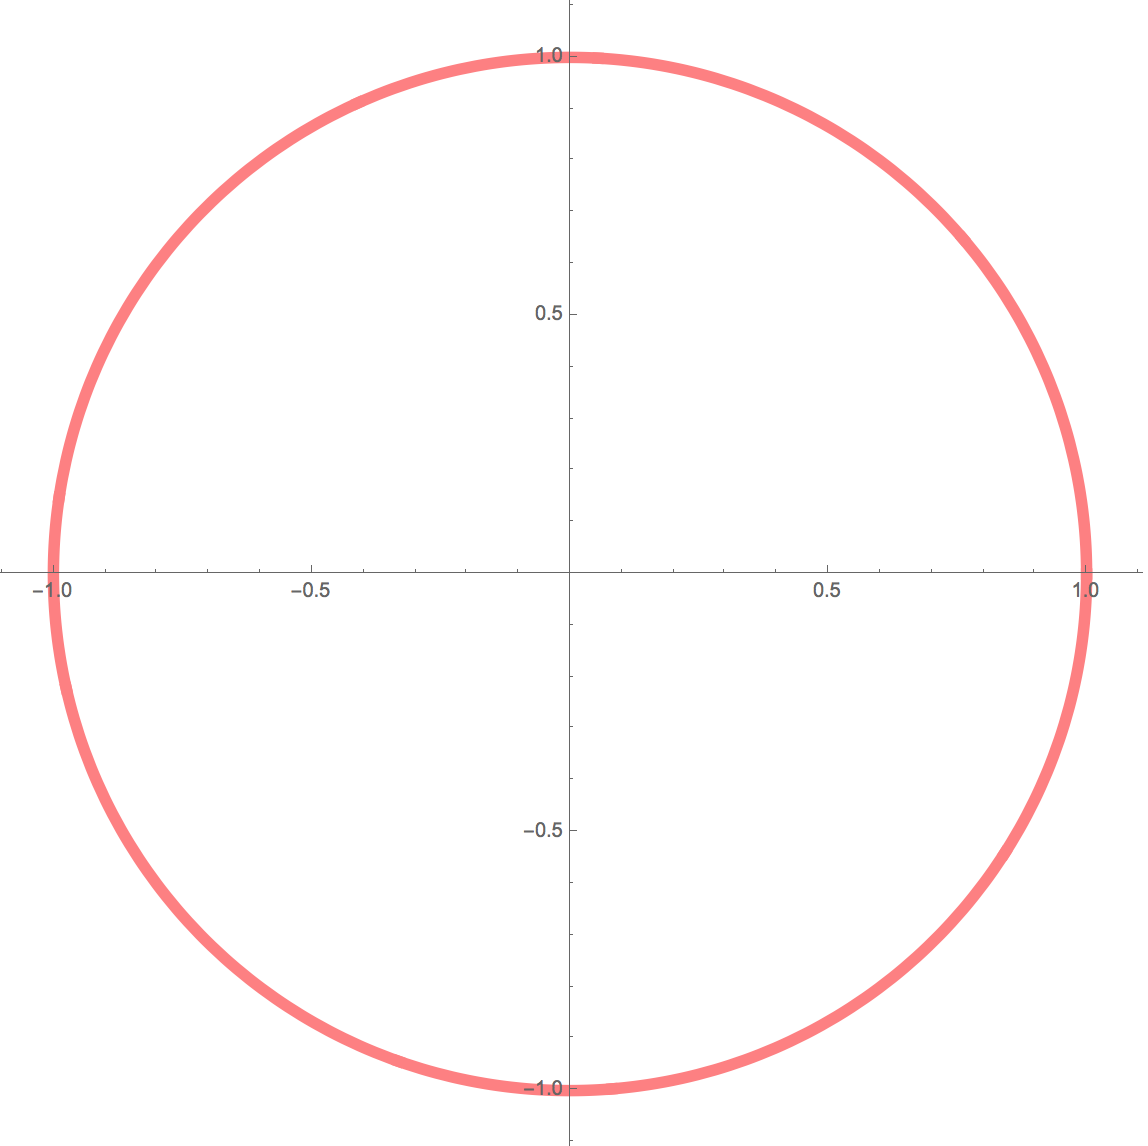
\includegraphics[scale=0.3]{arclength_circle.png}
\end{figure}

What about the path length of a helix? Note that one turn of a helix in three dimensions is just a circle in two dimensions that has been cut at one point and stretched.  Figure~\ref{fig:arclengthhelix} provides an illustration of two turns of a helix. (The stretching is what will make the path length of a helix different from that of the unit circle.) A helix is parametrized by the following function, $\mathbf{f}(t) = (\cot{t}, \sin{t}, t)$. Applying the definition for path length as before we can find two turns of a helix as follows,
\[
\int_{0}^{4\pi} \norm{\mathbf{f}'(t)} \ dt = \int_{0}^{4\pi} \sqrt{2} \ dt =  [\sqrt{2}t]_{0}^{4\pi} \approx 17.77
\]

Notice how the path length of two revolutions around the unit circle is equal to $4\pi$, which is less than the path length of two turns of a helix by a factor of $\sqrt{2}$. \\

\begin{figure}[h]
\centering
\caption{Plot of $\mathbf{f}(t) = (\cos{t}, \sin{t}, t)$ where $0\leq t\leq 4\pi$}
\label{fig:arclengthhelix}
\indent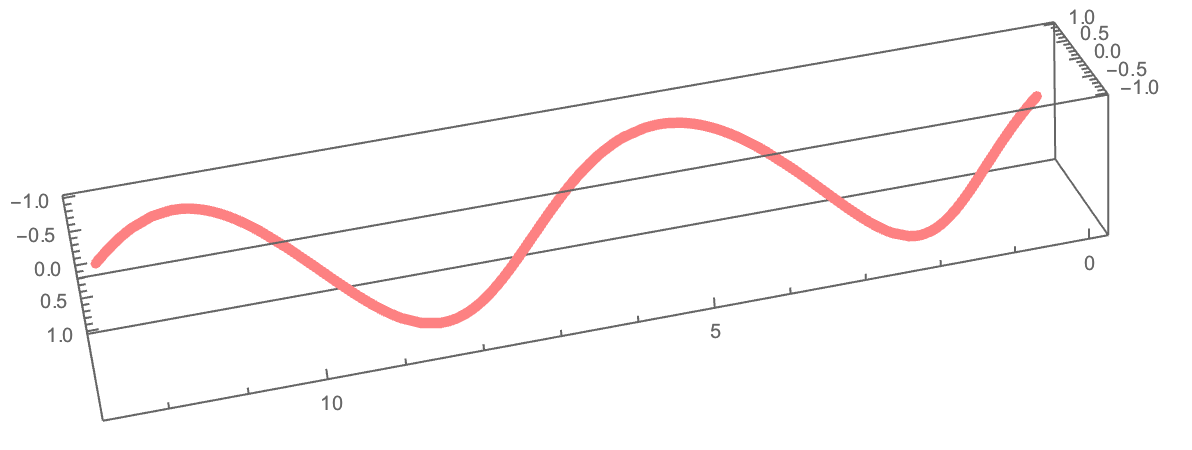
\includegraphics[scale=0.7]{arclength_helix.png}
\end{figure}

It might be obvious now, but a helix does not represent a spiral in three dimensions. A spiral in three dimension takes more of conical, rather than cylindrical, shape. It is as if you were to lift up a two dimensional spiral from the center and pull it off the page into three dimensions. See Figure~\ref{fig:arclengthexample} for a two dimensional spiral and Figure~\ref{fig:spiral3d} for a spiral in three dimensions. \\

The typical parametrized function that defines a spiral, $\mathbf{f}(t) = (t\cos{t}, t\sin{t})$. One turn of the spiral corresponds to $t$ going from $0$ to $2\pi$ (see Figure~\ref{fig:arclengthexample}). The length of this path can be found using the definition above. First find the gradient,
\[
\mathbf{f}'(t) = (\cos{t}-t\sin{t}, \sin{t}+t\cos{t})
\]
Now find the magnitude of the gradient,
\[
\norm{\mathbf{f}'(t)} = \sqrt{\cos{^2t} + \sin{^2t} + t^2(\cos{^2t} + \sin{^2t})} = \sqrt{1+t^2}
\]
Now find the definite integral,
\[
\int_{0}^{2\pi} \norm{\mathbf{f}'(t)}  = \int_{0}^{2\pi}  \sqrt{1+t^2}\ dt = \pi\sqrt{1+4\pi^2} + \frac{\arcsin{(2\pi)}}{2} \approx 21.26
\]
which gives us the path length of one turn of the spiral defined by $\mathbf{f}(t)$. (You can use trig substitution and/or a mathematical computation program to get to the answer.)

\begin{figure}[h]
\centering
\caption{Plot of $\mathbf{f}(t) = (t\cos{t}, t\sin{t})$ where $0\leq t\leq 2\pi$}
\label{fig:arclengthexample}
\indent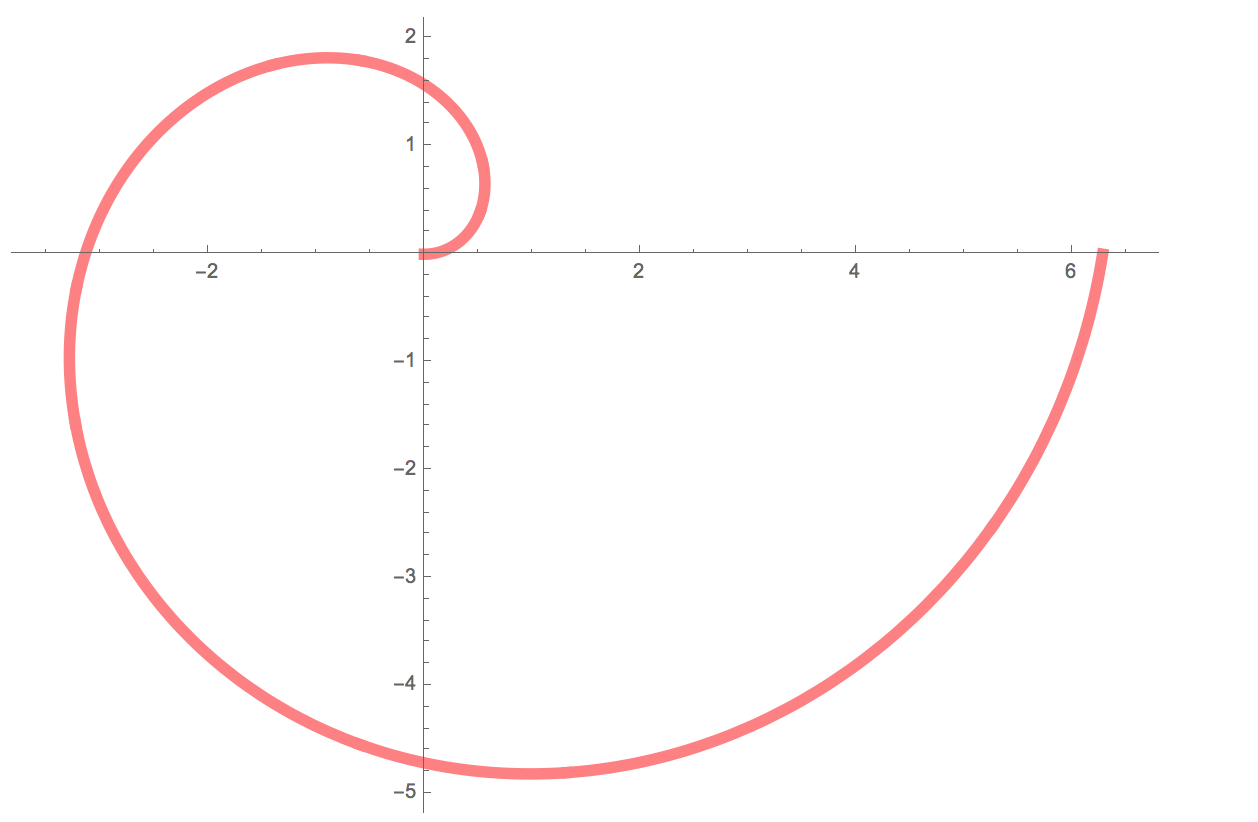
\includegraphics[scale=0.4]{arclength_spiral.png}
\end{figure}

\begin{figure}[h]
\centering
\caption{Plot of $\mathbf{f}(t) = (t\cos{t}, t\sin{t}, t)$ where $0\leq t\leq 12\pi$}
\label{fig:spiral3d}
\indent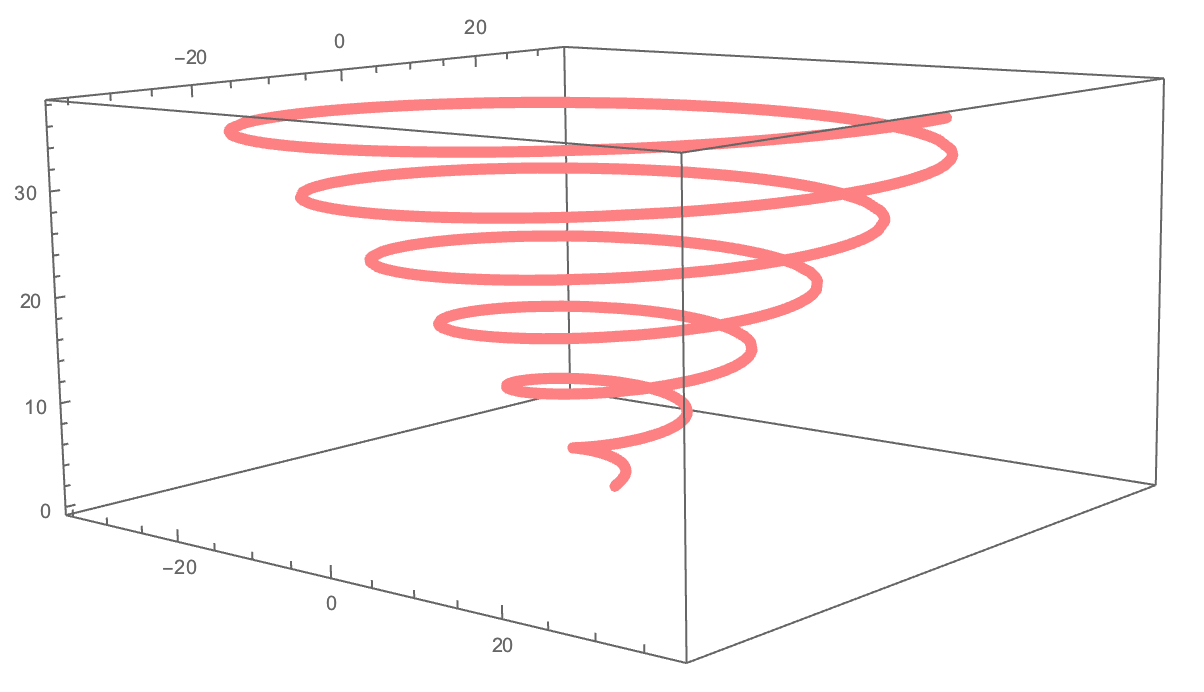
\includegraphics[scale=0.4]{spiral3d.png}
\end{figure}



\subsection{Iterated Integrals}

Recall that the definition of the definite integral for single variable functions was interpreted as the area under the curve between two bounds. \\

\begin{framed}
\textbf{Single Variable Integration}
\[
\int_a^b f(x) dx = \lim_{n\rightarrow\infty}\sum_{i=1}^n f(x_i)\Delta x_n
\]
where, $f$ is continuous, $f:U\subset\real\rightarrow\real$, $\Delta x_n=\frac{b-a}{n}$ is the length of each of the $n$ subintervals that we divide the domain space into, and $x_i = (a+i)\Delta x_n$.
\end{framed}

Note that $\Delta x_n$ is constant, whereas $f(x_i)$ is not.\\

\emph{Double integrals} are the two dimensional version of definite integrals for single variable functions. An application of double integrals is that they allow you to determine the volume under a surface in $\real^3$ space.\\

We can extend the definition of the single integral to the double integral. \\

\begin{framed}
\textbf{Double Integral} \\
Let $f:R\subset\real^2\rightarrow\real$. Where $R=[a,b]\times[c,d]$ (i.e. $R$ is a rectangle). Then the double integral is,
\[
\int\int_R f(x,y)dA = \lim_{n,m\rightarrow\infty}\sum_{i=1}^n\sum_{j=1}^m f(x_i,y_j)\Delta x_i \Delta y_j
\] 
\[
\int\int_R f(x,y)dA = \lim_{n \rightarrow \infty} \sum_{(x_i,y_i)\in R} f(x_i,y_i) \Delta A_n
\]
 Here, $\Delta A$ is the area differential. Also, let $\Delta x = \frac{b-a}{n}$ and let $\Delta y = \frac{d-c}{n}$, where $n$ represents the number of equal subdivisions of the region $R$. Finally, $A_n = \Delta x \Delta y$. Note that the concept of the double integral can be generalized to a non rectangular region. 
 \end{framed}

The double integral can be evaluated using the process of iteration. Specifically, if $f(x,y)$ is continuous and the region $R=\{(x,y)|a\leq x\leq b, g_1(x) \leq y \leq g_2(x)\}$ where $g_1(x)$ and $g_2(x)$ are the lower and upper limits of the integral with respect to variable $y$, respectively, then,
\[
\int\int_R f(x,y)dA = \int_a^n\int_{g_1(x)}^{g_2(x)} f(x,y) dydx
\]

 For example, in order to evaluate the integral,
\[
\int_0^1\int_{1-x}^{1+x} xy\ dydx
\]
we first evaluate the inner integral $\int_{1-x}^{1+x}$ with respect to $y$ and then the outer integral $\int_0^1$ with respect to x. This will give us,
\begin{align*}
\int_0^1\int_{1-x}^{1+x} xy\ dydx &= \int_0^1\left[ \frac{xy^2}{2} \right]_{1-x}^{1+x} dx \\
&= \int_0^1 2x\ dx \\
&= \left[ x^2 \right]_0^1 \\
&= 1
\end{align*} 

Figure~\ref{fig:iteratedintegralexample} is a graph of the function $f(x,y) = xy$ on which the double integral was performed. The double integral evaluates the area under this surface. 

\begin{figure}[H]
\centering
\caption{Plot of $f(x,y) = xy$}
\label{fig:iteratedintegralexample}
\indent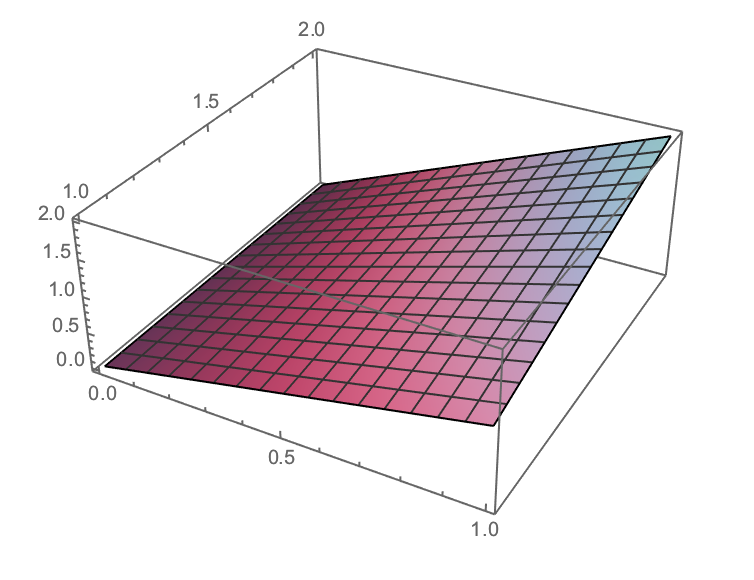
\includegraphics[scale=0.5]{iterated_integral_example.png}
\end{figure}

\subsection{Line Integrals}

 We will first define the \emph{scalar line integral} and then the \emph{vector field line integral}. With the examples that follow, the interpretation of what a line integral is will be clear.  \\

 Consider a continuous function $f:U\subset\real^2\rightarrow\real$ over a smooth path $C$. The scalar line integral of $f$ along path $C$ is,
\[
\int_C f(x,y) ds = \lim_{n\rightarrow\infty} \sum_{i=1}^n f(x_i,y_i) \Delta s_i
\]
where $\Delta s_i,\ldots,\Delta s_n$ represents the path $C$ divided into $n$ subarcs. Analogous to the integral of a single variable function, here we are dividing the path into $n$ subarcs and taking the limit as these partitions become infinitesimally small. The scalar line integral evaluates the area under the function along the curve. \\ 

 A more appropriate interpretation of the line integral is how it describes the relationship between the a vector field and a path on a vector field. The line integral is just the sum of the dot products of the vector field (i.e. a given point in the vector field) and the tangent vector along the path prescribed by the function (at that same point). \\

 To formalize this interpretation, consider the vector field $\mathbf{F}:U\subset\real^n\rightarrow\real^n$ and the smooth path $C$ in $U$ which is parameterized by $\mathbf{x}=\mathbf{f}(t),\ a\leq t\leq b$. $\mathbf{F}$ takes the value $\mathbf{F}(\mathbf{f}(t))$ at each point on path $C$. At each change in $t$ the objects change in position on path $C$ is given by $\mathbf{f}'(x)\Delta t$. It follows that 
\[
\mathbf{F}(\mathbf{f}(t)) \cdot \mathbf{f}'(t)\Delta t
\]
is the work done by the vector field $\mathbf{F}$ on an object on path $C$ in the short interval $\Delta t$. Here work is defined as the product between the force exerted on an object at time $t$, which is given by $\mathbf{F}(\mathbf{f}(t))$, and the distance the object travels from time $t$ to $t+\Delta t$, which is given by $\mathbf{f}'(t)\Delta t$.\\

 Figure~\ref{fig:vectorfieldexample2} provides an example of a vector field with a path overlaid. If we drop an object on the path then the properties of the vector field will move it along the path. \\

\begin{figure}[h]
\centering
\caption{Vector Field with a Path}
\label{fig:vectorfieldexample2}
\indent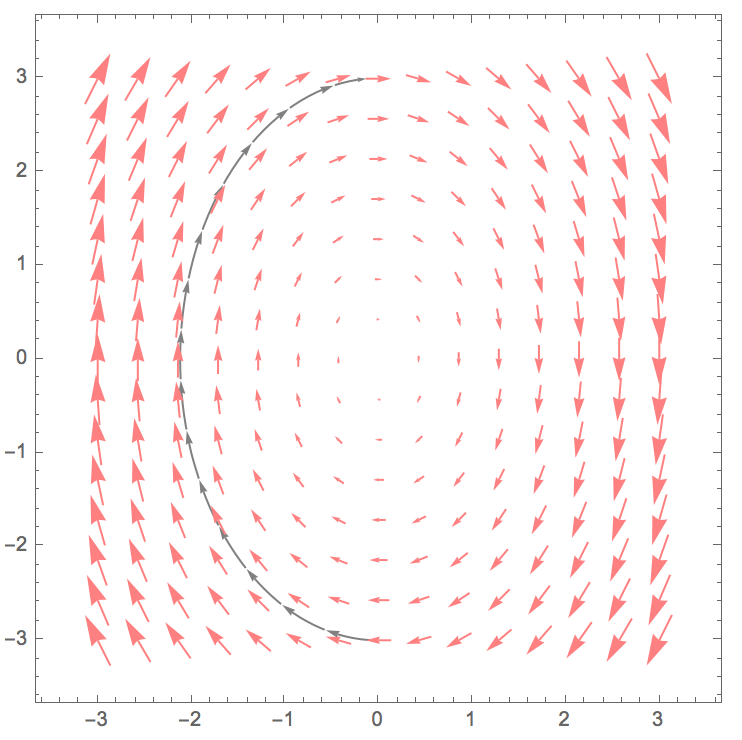
\includegraphics[scale=0.7]{vector_field_example2.png}
\end{figure}

 If we are interested in finding the total amount of work done by an object on the path then we can simply take the sum over all the changes in $t$,
\[
\sum_{i=1}^{n} \mathbf{F}(\mathbf{f}(t)) \cdot \mathbf{f}'(t)\Delta t_i
\]

 The sum above is the discrete approximation of the following integral,
\[
\int_{i=1}^{n} \mathbf{F}(\mathbf{f}(t)) \cdot \mathbf{f}'(t)\  dt
\]

\begin{framed}
\textbf{Line Integral} \\
 Formally, the \emph{line integral} or \emph{path integral} of a continuous vector field $\mathbf{F}$ over a smooth path $C$ is,
\[
\int_{C} \mathbf{F}\cdot d\mathbf{x} = \int_{a}^{b} \mathbf{F}(\mathbf{f}(t)) \cdot \mathbf{f}'(t)\  dt
\]
where $\mathbf{f}(t)$ is the parametrization of $C$, and $a\leq t\leq b$. \\
\end{framed}

 As an example, consider the vector field $\mathbf{F}(x,y) = (x+2y, x^2-y^2)$ and let the path consist of the line segments $(3,-1)$ to $(1,-1)$ and $(1,-1)$ to $(1,2)$. This is illustrated in Figure~\ref{fig:lineintegralexample}.

\begin{figure}[h]
\centering
\caption{Piecewise Smooth Path}
\label{fig:lineintegralexample}
\indent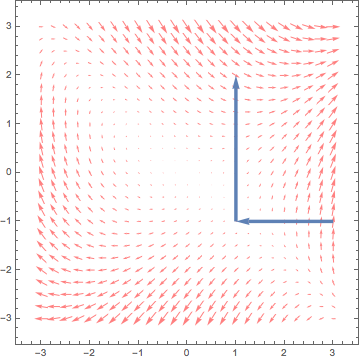
\includegraphics[scale=0.6]{line_integral_example.png}
\end{figure}

 In order to evaluate the line integral of the vector field over the path we have to first parameterize the path by a single variable $t$. The horizontal line segment can be defined as $(x,-1)$ and the vertical line segment can be defined as $(1,y)$.  Therefore, for the horizontal line segment $h$ we have the parametrization,
\[
L_h(t) = (t,-1)
\] 
and for the vertical line segment $v$ we have,
\[
L_v(t) = (1,t)
\]
Using the definition of the line integral (and evaluating each path separately) gives us the following,
\begin{align*}
\int_{1}^{3} \mathbf{F}(L_h(t)) \cdot L'_h(t) &= \int_{1}^{3} (t-2,t^2-1) \cdot (1,0) = \int_{1}^{3} t-2 \\
\int_{-1}^{2} \mathbf{F}(L_v(t)) \cdot L'_v(t) &= \int_{-1}^{2} (1-2t,1-t^2) \cdot (0,1) = \int_{-1}^{2} 1-t^2
\end{align*}
Taking the integral we have,
\begin{align*}
\int_{1}^{3} t-2 &= \left[ \frac{t^2}{2} - 2t \right]_1^3 = 0 \\
\int_{-1}^{2} 1-t^2 &=  \left[ t - \frac{t^3}{3} \right]_{-1}^2 = 0
\end{align*}
Recall that the line integral of the vector field along the path $(3,-1)$ to $(1,-1)$ to $(1,2)$ is the sum of the line integral along $(3,-1)$ to $(1,-1)$ and the line integral along $(1,-1)$ to $(1,2)$. Therefore, the line integral evaluated is zero. In the physics sense the work done by the force field on the object is zero along the path. This makes sense if you identify the orthogonality between the vector field and the tangent vector to the path in Figure~\ref{fig:lineintegralexample}. As the object travels along the path, the dot product between the tangent vector and the vector defined by the vector field at each point is equal to zero. Therefore, the sum of these dot products (i.e. the line integral) must also be zero. \\

 If the vectors defined by the vector field are not perpendicular to the tangent vectors of the path at each point $t$ then there is either positive work (the vector field is directing the object along the path, or there is negative work (the vector field is directing the object in a direction that opposes the path. \\

 In Figure~\ref{fig:lineintegralexample2} a new path has been introduced to the vector field and path given in Figure~\ref{fig:lineintegralexample}. This new path is defined by the function $f(x) = \frac{3}{2}x + \frac{7}{2}$, where $1\leq x \leq3$. \\

\begin{figure}[h]
\centering
\caption{A Piecewise Smooth Path and a Smooth Path}
\label{fig:lineintegralexample2}
\indent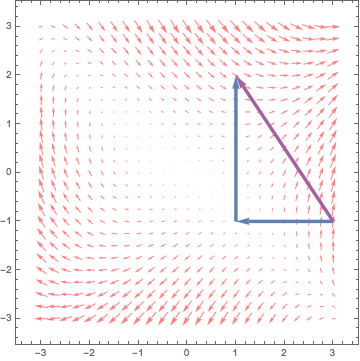
\includegraphics[scale=0.6]{line_integral_example2.png}
\end{figure}

 We can evaluate the work done by the vector field along this path. First note that the curve has already been parametrized in terms of one variable: $f(x) = -\frac{3}{2}x + \frac{7}{2} \Leftrightarrow f(t) = -\frac{3}{2}t + \frac{7}{2}$. The vector field is identical to the previous example and is defined as $\mathbf{F}(x,y) = (x+2y, x^2-y^2)$. We can define $f(t)$ as the vector valued function $\mathbf{f}(t) = (t,-\frac{3}{2}t+\frac{7}{2})$. Now we can evaluate the vector field at this function, \\
\[
\mathbf{F}(\mathbf{f}(t)) = \left( -2t + 7, -\frac{5}{4}t^2 + \frac{42}{4}t - \frac{49}{4} \right)
\]
and we can evaluate the derivative of the vector valued path function,
\[
\mathbf{f}'(t) = \left( 1, -\frac{3}{2} \right)
\]

 Now we have all the components required to evaluate the line integral,
\begin{align*}
\int_1^3 \mathbf{F}(\mathbf{f}(t))\cdot\mathbf{f}'(t) &= \int_1^3  \frac{15}{8}t^2 + \frac{142}{8}t + \frac{203}{8} \ dt\\
&= \left[ \frac{5}{8}t^3 + \frac{71}{8}t^2 + \frac{203}{8}t \right]_1^3 \\
&= -4
\end{align*}

 So with regard to this path, the work done by the vector field along the path is negative.  Looking at Figure~\ref{fig:lineintegralexample2} this seems like the appropriate conclusion since there are few points along the path at which the dot product between the vector field and the gradient along the path would be positive or zero.\\

\pagebreak
\section{Fundamental Theorems}

\subsection{Fundamental Theorem of Calculus}

From single variable calculus we have the \emph{Fundamental Theorem of Calculus}, which connects integration to differentiation by showing that integration is anti-differentiation. \\

Let $f(x)$ be a continuous function. From the definition of integration we can define the area under a curve as a function of one of the integral boundaries,
\[
A(x) = \int_{a}^{x} f(t) dt
\]
Using the definition of differentiation we can then define the rate of change of this area,
\[
\frac{d}{dx}A(x) = \lim_{h\rightarrow0} \frac{A(x+h)-A(x)}{h} = f(t)
\]
It follows that,
\[
\frac{d}{dx} \int_{a}^{x} f(t) dt = f(t)
\]
This is the first part of the Fundamental Theorem of Calculus and shows that integration is just anti-differentiation. With respect to the notation above, $A(x)$ is the anti-derivative of $f(x)$. This is illustrated in Figure~\ref{fig:ftc1}. \\

% Fundamental Theorem of Calculus - Part 1
\begin{figure}[h]
\centering
\caption{Fundamental theorem of Calculus - Part 1}
\label{fig:ftc1}
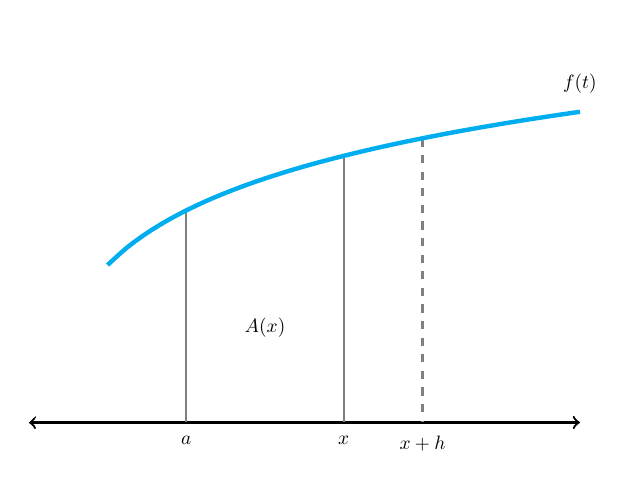
\begin{tikzpicture}[scale=1, every node/.style={scale=0.7}]
% Draw axes
\draw[<->, thick] (0,0)--(7,0);
\draw[<->, thick, white] (0,0)--(0,5);
% Draw vectors
\draw[thick, gray] (2,2.69)--(2,0);
\draw[thick, gray] (4,3.38)--(4,0);
\draw[dashed, thick, gray] (5,3.609)--(5,0);
\draw[domain=1:7,smooth,variable=\x, ultra thick, cyan] plot ({\x},{2+ln(\x)});
% Draw labels
\node [label=above:{$f(t)$}] at (7,4) {};
\node [label=below:{$a$}] at (2,0) {};
\node [label=below:{$x$}] at (4,0) {};
\node [label=below:{$x+h$}] at (5,0) {};
\node [label=below:{$A(x)$}] at (3,1.5) {};
\end{tikzpicture}
\end{figure}

From integration we know that,
\[
\int_{a}^{b} f(t)dt = A(b) - A(a) 
\] 
where $a<b$, $A(b)$ and $A(a)$ are indefinite integrals (which is analogous to saying they are anti-derivatives of $f(b)$ and $f(a)$, respectively). Substituting the fact that $A'(x) = f(t)$ from the first part of the fundamental theorem we have,
\[
\int_{a}^{b} A'(x)dx = A(b) - A(a) 
\]

This is the second part of the Fundamental Theorem of Calculus. It uses the first part of the fundamental theorem to show that integration evaluates the area under a curve between the two integration bounds. This is illustrated in Figure~\ref{fig:ftc2}.

% Fundamental Theorem of Calculus - Part 2
\begin{figure}[h]
\centering
\caption{Fundamental Theorem of Calculus - Part 2}
\label{fig:ftc2}
\begin{tikzpicture}[scale=1, every node/.style={scale=0.7}]
% Draw axes
\draw[<->, thick] (0,0)--(7,0);
\draw[<->, thick, white] (0,0)--(0,5);
% Draw vectors
\draw[thick, gray] (2,2.69)--(2,0);
\draw[thick, gray] (4,3.38)--(4,0);
\draw[domain=1:7,smooth,variable=\x, ultra thick, cyan] plot ({\x},{2+ln(\x)});
% Draw labels
\node [label=above:{$f(t)$}] at (7,4) {};
\node [label=below:{$a$}] at (2,0) {};
\node [label=below:{$b$}] at (4,0) {};
\node [label=below:{$A(x)$}] at (3,1.5) {};
\end{tikzpicture}
\end{figure}

\subsection{Fundamental Theorem of Line Integrals}

Intuitively, one might think that some paths that take an object from point A to point B will require more/less work than other paths, as illustrated in Figure~\ref{fig:lineintegralexample3}. However, for certain vector fields this not the case. If the vector field is the gradient of a scalar valued function then it is path independent (i.e. all path that takes you from point A to point B will yield the identical amount of work). This is established in the \emph{Fundamental Theorem of Line Integrals}.\\

This fundamental theorem requires the property of \emph{connected sets}. A set  $A\in\real^n$ is connected if, for any two points $\mathbf{a}$ and $\mathbf{b}$ in $A$, there exists a continuous path lying in $A$ that joins the points $\mathbf{a}$ and $\mathbf{b}$. \\

\begin{framed}
\textbf{Fundamental Theorem of Line Integrals}\\
Let $U\subset\real^n$ be an open connected set and let $f:U\rightarrow\real$ be a function whose gradient is continuous on $U$. If $C$ is any smooth continuous path lying in $U$ that joins points $\mathbf{a}$ and $\mathbf{b}$ then,
\[
\int_C \grad f(\mathbf{x}) \cdot d\mathbf{x} = f(\mathbf{b})-f(\mathbf{a})
\]
\end{framed}

To sketch out the proof, parametrize $C$ by $\mathbf{g}(t)=\mathbf{x}$, where $\alpha\leq t\leq\beta$, and define $\mathbf{g}(\alpha)=\mathbf{a}$ and $\mathbf{g}(\beta)=\mathbf{b}$. \\ 

As an aside, recall that parametrization means that we are taking the scalar valued function with multiple variables $f(\mathbf{x})$ and translating it into the vector valued function $\mathbf{g}(t)$ with a single variable. For example we are taking the following function,
\[
f(\mathbf{x})=f(x_1,x_2) = x_1 + 2x_1x_2
\]
and parametrizing it to,
\[
\mathbf{g}(t) = \begin{bmatrix}t + 2x_2t & x_1 + 2x_1t\end{bmatrix}
\]
Notice that,
\[
\grad f(\mathbf{x}) = \frac{d}{dt}\mathbf{g}(t) =  \begin{bmatrix}1 + 2x_2 & 2x_1 \end{bmatrix}
\]

Back to the proof. Applying the parametrization we have,
\[
\int_C \grad f(\mathbf{x}) \cdot d\mathbf{x} = \int_{\alpha}^{\beta} \grad f(\mathbf{g}(t)) dt
\]
Since we are taking the gradient with respect to only one variable, the above is identical to,
\[
\int_C \grad f(\mathbf{x}) \cdot d\mathbf{x} = \int_{\alpha}^{\beta} \frac{d}{dt} f(\mathbf{g}(t)) dt
\]
Applying the Fundamental Theorem of Calculus (second part) we have,
\begin{align*}
\int_C \grad f(\mathbf{x}) \cdot d\mathbf{x} &= \int_{\alpha}^{\beta} \frac{d}{dt} f(\mathbf{g}(t)) dt \\
&= f(\mathbf{g}(\beta))-f(\mathbf{g}(\alpha)) \\
&= f(\mathbf{b})-f(\mathbf{a}) \\
\end{align*}

The Fundamental Theorem of Line Integrals relied on the assumption that $f$ is a scalar valued function with a continuous gradient on $U$. In other words this assumption is saying that the vector field $\mathbf{F}$ must be the gradient of some function, i.e. $\mathbf{F} = \grad f(\mathbf{x})$. If this is true then the line integral (i.e. the work done by the object along the path) is simply the difference between the endpoints evaluated at the function $f$ (known as the \emph{potential function}) whose gradient is $\mathbf{F}$. Such vector fields are known as \emph{conservative vector fields} or \emph{path independent vector fields}. \\

For example, consider the vector field,
\[
\mathbf{F}=(\underbrace{1+2x_2}_{F_1}, \underbrace{2x_1+2x_2}_{F_2})
\]
We can determine the potential function $f$ of this vector field by finding,
\begin{align*}
\int F_1 dx_1 &= x_1 + 2x_1x_2 + C \\
\int F_2 dx_2 &= 2x_1x_2 + x_2^2 + C
\end{align*}
The common terms for $F_1$ and $F_2$ are $2x_1x_2+C$. In order to equate $F_1$ and $F_2$ we need to add $x_2^2$ to $F_1$ and add $x_1$ to $F_2$. This gives us the potential function of $\mathbf{F}$
\[
f(\mathbf{x}) = x_1 + 2x_1x_2 + x_2^2
\]
As a check notice that $\mathbf{F}=\grad f$. \\

This was pretty straightforward since the vector field in the above example was conservative by design. Unfortunately, it is not always easy to determine by inspection whether a vector field is conservative. 

The Fundamental Theorem of Line Integrals gives us a quick way to evaluate a line integral. However, it relies on the assumption that the vector field is conservative and we need a way to check that this true. \\

One check is that if $\oint_C \mathbf{F} \cdot d\mathbf{x} = 0$ for all closed paths $C$ that lie in the domain then the vector field $\mathbf{F}$ is conservative. This is an arduous task since it requires evaluating \emph{all} closed paths in the domain to rule out the possibility that $\oint_C \mathbf{F} \cdot d\mathbf{x} \neq 0$. \\

The general check is to evaluate the Jacobian of the vector field and determine whether it is symmetric. If it is then the vector field is conservative. Recall that a matrix $\mathbf{M}$ is symmetric if $\mathbf{M}=\mathbf{M}^\top$. \\

Formally, let $U\in\real^n$ be a simply connected open set and let $\mathbf{F}:U\rightarrow\real^n$ be a continuously differentiable vector field. The vector field $\mathbf{F}$ is conservative if and only if the Jacobian matrix $J\mathbf{F}$ is symmetric, i.e. $J\mathbf{F}=(J\mathbf{F})^T$. (Note that a \emph{simply connected set} is a set that has no holes (i.e. gaps) through it.) \\

Figure ~\ref{fig:lineintegralexample3} illustrates the vector field $\mathbf{F}(x,y) = (x+6xy, 3y^2+3x^2)$. This is a conservative vector field since,
\[
J\mathbf{F} =
\begin{bmatrix}
1+6y & 6x \\
6x & 6y
\end{bmatrix}
=
(J\mathbf{F})^T
\]

\begin{figure}[h]
\centering
\caption{Path Independence on a Conservative Vector Field}
\label{fig:lineintegralexample3}
\indent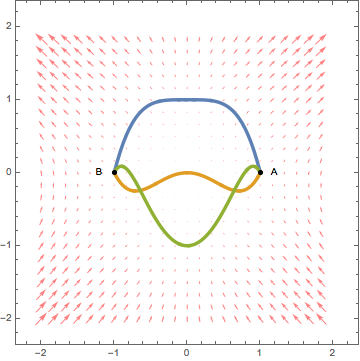
\includegraphics[scale=0.6]{line_integral_example3.png}
\end{figure}

Recall that this means any closed smooth continuous path has a line integral of zero. It also means that any path from point $A\ (1,0)$ to point $B\ (-1,0)$ will have an identical line integral. For example, the blue path is parametrized by the vector valued function $\mathbf{f}(t,1-t^4)$. In order to use the formula for evaluating line integrals we need,
\[
\mathbf{f}'(t) = (1,4t^3)
\]
and,
\[
\mathbf{F}(\mathbf{f}(t)) = (7t-6t^5, 3t^8-6t^4+3t^2+3)
\]
Now we can evaluate the line integral,
\[
\int^{-1}_{1}\mathbf{F}(\mathbf{f}(t))\cdot\mathbf{f}'(t) \ dt = \int^{-1}{1} 2t^{11}-24t^7+6t^5+12t^3+7t \ dt = 0
\]

Note that since we know that the vector field is conservative, we can apply the Fundamental Theorem of Line Integrals. In this case we have,
\[
\int^{-1}_{1}\mathbf{F}(\mathbf{f}(t))\cdot\mathbf{f}'(t) \ dt = f(B)-f(A) = \left[1-(-1)^4\right]-\left[1-(1)^4\right] = 0
\]

Since the vector field is conservative the path prescribed by the orange and green paths should also give us a line integral of zero. The function describing the orange path is $f(t)=t^4-t^2$ and the function of the green path is $\mathbf{f}(t) = -1+2t^2-t^6$. For the orange path the line integral is,
\[
\int^{-1}_{1}\mathbf{F}(\mathbf{f}(t))\cdot\mathbf{f}'(t) \ dt = f(B)-f(A) = \left[(-1)^4-(-1)^2\right]-\left[(1)^4-(1)^2\right] = 0
\]

By applying the Fundamental Theorem of Line Integrals, the same result can be obtained for the green path.


%\indent\includegraphics[scale=0.5]{3B3.png}


%CODE
% \pagebreak
% \section*{Code}
%\texttt{\lstinputlisting{HW7.R}}

\end{document}